\documentclass[journal,twoside]{IEEEtran}
\usepackage{mathptmx}  % Times Roman with math support (BasicTeX compatible)
\usepackage{helvet}     % Helvetica for sans-serif

\usepackage{amsmath,amssymb,amsfonts}
\usepackage{graphicx}
\usepackage{textcomp}
\usepackage{xcolor}
\usepackage{booktabs}
\usepackage{tikz}
\usetikzlibrary{shapes.geometric, arrows.meta, positioning, fit, backgrounds, calc}
\usepackage{hyperref}

\hypersetup{
    colorlinks=true,
    linkcolor=blue!70!black,
    citecolor=blue!70!black,
    urlcolor=blue!70!black,
}

\newcommand{\VocSixG}{Voc-6G}

\begin{document}

\title{Voc-6G: A CyberTwin-Enabled Intelligent Task Migration Framework for 6G mmWave Vehicular Edge Computing}

\author{
\IEEEauthorblockN{Anonymous Authors}
\IEEEauthorblockA{Manuscript under review}
}

\markboth{IEEE Access}{Author et al.: Voc-6G CyberTwin-Enabled Task Migration for 6G mmWave Vehicular Edge Computing}

\maketitle

\begin{abstract}
The proliferation of connected and autonomous vehicles in 6G networks demands ultra-reliable, low-latency computation offloading, yet existing task migration frameworks rely on ad-hoc synthetic simulations that fail to capture the stochastic complexity of real vehicular environments. This paper presents \VocSixG{}, a CyberTwin-enabled intelligent task migration framework for 6G mmWave vehicular edge computing. The CyberTwin layer maintains synchronized digital replicas of 300 vehicles, 25 Roadside Units (RSUs), and 8 Multi-access Edge Computing (MEC) servers operating at 28\,GHz, from which 40,000 migration decision records are harvested for training and evaluation. \VocSixG{} integrates four synergistic modules: (i) an LSTM-based predictive module that forecasts dwell time, signal quality degradation, edge congestion, and migration failure probability from historical observation sequences; (ii) a trust scoring and anomaly detection module leveraging z-score analysis and composite reliability metrics to identify malicious or degraded edge nodes; (iii) a migration policy engine employing Behavioral Cloning (BC) for supervised imitation learning and Conservative Q-Learning (CQL) for offline reinforcement learning from logged migration decisions; and (iv) a Federated Learning layer using FedAvg and FedProx aggregation to enable privacy-preserving distributed training without centralizing raw data. A modified simulated annealing optimizer with a nonstandard acceptance criterion provides auxiliary hyperparameter tuning. Comprehensive experiments on 6,000 held-out test instances demonstrate that \VocSixG{} with leak-free trust-aware filtering achieves F1-Macro=0.9998, AUC-ROC=0.9998, while the federated variant maintains competitive performance (F1-Macro=0.9929) without data centralization. Multi-seed stability analysis across eight random seeds confirms a mean F1-Macro of $0.9925 \pm 0.0011$ for the BC variant, demonstrating robust generalization. A simple post-hoc trust filter achieves only F1=0.3906, confirming that trust must be integrated into the model architecture rather than applied as a post-processing step.\footnotemark
\end{abstract}

\begin{IEEEkeywords}
6G, Internet of Vehicles, CyberTwin, task migration, federated learning, mmWave, edge computing, offline reinforcement learning, trust management, LSTM
\end{IEEEkeywords}

\footnotetext{When trust scores are computed from the full training set, information leakage yields F1=1.0000 — this represents an upper bound artifact, not genuine generalization performance.}

%% ============================================================
%%  SECTION I: INTRODUCTION
%% ============================================================
\section{Introduction}
\label{sec:introduction}

The emergence of 6G wireless networks promises to fundamentally transform the Internet of Vehicles (IoV) by enabling high-capacity data rates, ultra-low latency communication, and massive device connectivity~\cite{zhang20206g, wu2020comprehensive}. A key enabling technology for 6G is the CyberTwin paradigm---a digital replica framework that maintains real-time synchronized models of physical vehicles, network infrastructure, and computational resources~\cite{liang2022cybertwin, hu2023cybertwin}. CyberTwins enable proactive resource orchestration by predicting future system states and pre-allocating resources before demand materializes, a capability essential for safety-critical vehicular applications such as autonomous driving, cooperative perception, and real-time traffic optimization~\cite{dai2021survey, zhang2022cybertwin}.

A central challenge in CyberTwin-enabled IoV is \emph{intelligent task migration}---the dynamic decision of whether to execute a computation task locally on the vehicle or offload it to a proximate edge node such as a Roadside Unit (RSU) or Multi-access Edge Computing (MEC) server~\cite{mach2019mobile, huang2021computation}. Unlike static offloading, task migration must account for the highly dynamic vehicular environment where vehicles traverse multiple network coverage zones at varying speeds, signal quality fluctuates rapidly due to mobility and urban canyon effects, and edge node availability and load change unpredictably~\cite{zhang2020mobile, abbas2020mobile}. A poor migration decision can result in task failure due to vehicle departure from the serving RSU's coverage area, deadline violations from unexpected latency spikes, or security breaches from offloading to compromised nodes.

Despite significant research efforts, existing task migration approaches suffer from three critical limitations. \textbf{First}, the vast majority of frameworks are evaluated using standalone synthetic simulators (e.g., NS-3, SUMO, or custom discrete-event simulators) that are not grounded in empirical data distributions, making it difficult to assess real-world deployability~\cite{hou2018mobile, sun2021toward}. \textbf{Second}, most approaches treat task migration as a single-armed optimization problem without integrating security considerations such as node trustworthiness, anomaly detection, or reliability scoring~\cite{wang2020resource, chen2022intelligent}. \textbf{Third}, privacy concerns are frequently overlooked; training a global migration model typically requires centralizing migration logs from all edge zones, exposing sensitive mobility and task data~\cite{wang2020federated, lim2021federated}.

To address these limitations, we propose \VocSixG{}, a CyberTwin-enabled intelligent task migration framework for 6G mmWave vehicular edge computing. The key contributions of this work are:

\begin{itemize}
    \item \textbf{CyberTwin-facilitated training data}: \VocSixG{} leverages a CyberTwin layer that maintains synchronized digital replicas of 300 vehicles, 25 RSUs, and 8 MEC servers. Training migration decisions are harvested from CyberTwin state logs, where the digital replicas reflect the operational characteristics of their physical counterparts. The CyberTwin computes signal propagation using the 3GPP UMi path loss model at $f_c=28$\,GHz, vehicle movement follows the statistical distributions of the CRAWDAD Cabspotting dataset, and MEC server utilization is modeled following ETSI MEC utilization profiles~\cite{etsi_mec003}. This approach grounds the evaluation in empirically-calibrated distributions while leveraging the CyberTwin's capacity for persistent state tracking and historical log collection.

    \item \textbf{LSTM-based predictive module}: A Long Short-Term Memory (LSTM) network forecasts four critical migration conditions---remaining dwell time, future RSRP, congestion level, and migration failure probability---enabling proactive rather than reactive migration decisions.

    \item \textbf{Trust scoring and anomaly detection}: A composite trust score integrates historical migration success rates, z-score-based latency anomaly detection, authentication failure penalties, and consecutive failure streak penalties to identify and filter unreliable or malicious edge nodes.

    \item \textbf{Offline learning policy}: Behavioral Cloning (BC) is employed as a supervised imitation learning approach within the broader offline learning framework, while Conservative Q-Learning (CQL) constitutes the proper offline reinforcement learning component that optimizes a value function with distributional shift mitigation. Both learn from logged CyberTwin migration decisions, with success-weighted sampling to prioritize high-quality transitions.

    \item \textbf{Federated Learning integration}: FedAvg and FedProx aggregation enable privacy-preserving distributed training across RSU and MEC zones. Only model parameter updates are shared, preserving raw data locality.

    \item \textbf{Modified simulated annealing optimizer}: A hyperparameter optimizer with a nonstandard acceptance criterion combining classical and heuristic elements provides auxiliary tuning and candidate node ranking refinement.
\end{itemize}

Experimental results demonstrate that \VocSixG{} with leak-free trust-aware filtering achieves strong classification on the held-out test set (F1-Macro=0.9998, AUC-ROC=0.9998), while the federated variant maintains strong performance (F1-Macro=0.9929) without requiring data centralization. Multi-seed stability analysis confirms robust generalization with a mean F1-Macro of $0.9925 \pm 0.0011$ for the BC variant across eight independent random seeds.

The remainder of this paper is organized as follows. Section~\ref{sec:related} reviews related work. Section~\ref{sec:architecture} presents the system architecture. Section~\ref{sec:implementation} details the implementation. Section~\ref{sec:experiments} describes the experimental evaluation. Section~\ref{sec:discussion} discusses findings and implications. Section~\ref{sec:conclusion} concludes the paper.


%% ============================================================
%%  SECTION II: RELATED WORK
%% ============================================================
\section{Related Work}
\label{sec:related}

\subsection{Vehicular Edge Computing and Task Offloading}

Task offloading in vehicular environments has been extensively studied as a means to augment the limited computational capacity of on-board vehicle systems. Early approaches focused on static computation offloading, where tasks are either executed locally or offloaded to a fixed edge server based on instantaneous resource availability~\cite{chen2019computation, mao2017mobile}. Zhang et al.~\cite{zhang2015energy} formulated energy-efficient offloading as a convex optimization problem, while Mao et al.~\cite{mao2017mobile} developed a Lyapunov optimization framework for dynamic task offloading in mobile edge computing. These foundational works established the theoretical underpinnings of mobile edge computation but did not address the unique challenges of vehicular environments, particularly the rapid topology changes caused by vehicle mobility.

More recent work has incorporated mobility prediction into offloading decisions. Sun et al.~\cite{sun2021toward} proposed a mobility-aware computation offloading framework that uses vehicle trajectory prediction to estimate remaining connection time, while Hou et al.~\cite{hou2018mobile} considered vehicle-to-vehicle (V2V) cooperation to extend the computation offloading window. However, these approaches rely on simplified mobility models or require continuous GPS tracking, which may not always be available due to urban canyon signal blockage. Furthermore, none of these approaches consider the trustworthiness of target edge nodes as a factor in the offloading decision.

The task migration problem is distinct from traditional computation offloading in that it must handle \emph{in-progress} task transfer between edge nodes as a vehicle moves through coverage zones, rather than a one-time offloading decision. This requires continuous monitoring of connection quality, proactive handover initiation, and state transfer mechanisms---none of which are addressed by static offloading formulations. \VocSixG{} addresses task migration specifically by incorporating dwell time prediction and proactive migration initiation through its predictive module.

Huang et al.~\cite{huang2021computation} proposed a mobility-aware computation offloading scheme that predicts vehicle trajectories to optimize task scheduling. Sun et al.~\cite{sun2021drl} developed a joint task offloading and resource allocation framework using deep reinforcement learning. Zhang et al.~\cite{ref_offload1} addressed computation offloading for 6G edge computing with a joint optimization formulation. However, these approaches primarily rely on standalone simulated environments and do not incorporate CyberTwin-facilitated data generation or security-aware trust mechanisms.

\subsection{6G and CyberTwin for IoV}

The 6G vision extends beyond enhanced connectivity to encompass intelligence, sustainability, and digital-physical convergence~\cite{zhang20206g, wu2020comprehensive}. CyberTwin, as a key enabling technology for 6G, creates digital replicas of physical entities that enable predictive management and optimization~\cite{liang2022cybertwin}. Liang et al.~\cite{liang2022cybertwin} introduced the concept of CyberTwin-assisted network management for 6G, while Hu et al.~\cite{hu2023cybertwin} explored CyberTwin-based resource allocation in vehicular networks. Zhang et al.~\cite{zhang2022cybertwin} proposed a CyberTwin-empowered edge computing framework that predicts user demands and pre-provisions resources. Chen et al.~\cite{ref_dtIoV} presented a digital twin architecture for IoV from a 6G perspective. Our work extends these concepts by implementing a CyberTwin layer that maintains persistent synchronized digital replicas of vehicles, RSUs, and MEC servers, enabling continuous monitoring and historical log collection from which migration training data is harvested.

\subsection{Federated Learning for Edge Computing}

Federated Learning (FL) has emerged as a promising paradigm for privacy-preserving model training in distributed environments~\cite{mcmahan2017fedavg, kairouz2021advances}. In the context of vehicular edge computing, Wang et al.~\cite{wang2020federated} proposed a federated learning approach for resource allocation, while Lim et al.~\cite{lim2021federated} developed FedProx to handle data heterogeneity across edge clients. Zhang et al.~\cite{zhang2021federated} applied FL to collaborative task offloading in vehicular fog computing. Lim et al.~\cite{ref_fl_edge} surveyed federated learning for edge intelligence, identifying key challenges in resource-constrained deployments. However, these works typically assume simplified network models and do not integrate trust-aware security mechanisms with federated training for the specific task migration use case.

\subsection{Trust Management and Security in IoV}

Trust management is critical for secure task migration in IoV, where edge nodes may be compromised or unreliable. Various trust frameworks have been proposed, ranging from reputation-based systems~\cite{li2021trust} to blockchain-enabled trust mechanisms~\cite{zhang2020trust}. Chen et al.~\cite{chen2022intelligent} developed an intelligent trust management scheme for edge computing, while Xia et al.~\cite{xia2021security} explored security and privacy challenges in 6G-enabled IoV.

Recent work has advanced trust management for vehicular networks along several dimensions. Zhang et al.~\cite{zhang2023trust_composite} proposed a composite trust metric framework for vehicular networks that integrates multi-source reliability indicators with weighted aggregation, demonstrating improved accuracy over single-signal trust models. Li et al.~\cite{li2022trust_multidim} introduced multi-dimensional trust scoring augmented with z-score-based anomaly detection for identifying malicious edge nodes in V2X communication, showing that statistical anomaly detection significantly reduces false trust assignments under distribution shift. Wang et al.~\cite{wang2023trust_blockchain} developed a blockchain-empowered trust management scheme for edge computing that provides tamper-proof trust record storage and consensus-based trust aggregation, addressing the single-point-of-failure vulnerability in centralized trust architectures. Chen et al.~\cite{chen2024trust_federated} proposed a federated trust management framework for IoV that enables collaborative trust model training without sharing raw interaction data, achieving comparable trust accuracy to centralized approaches while preserving privacy across network operators.

Our approach builds upon these advances by integrating composite trust scoring directly into the migration decision pipeline through a multi-faceted metric that combines historical reliability, latency anomaly detection, authentication penalties, and failure streak analysis.

\subsection{Offline Reinforcement Learning for Network Optimization}

Offline RL learns policies from pre-collected datasets without online interaction, making it suitable for environments where real-time exploration is costly or risky~\cite{levine2020offline, fujimoto2019off}. This is particularly relevant for vehicular networks, where online exploration would require executing potentially suboptimal migration decisions on live traffic---a practice that could degrade user experience or violate safety constraints. Kumar et al.~\cite{kumar2020cql} proposed Conservative Q-Learning (CQL) to address the distributional shift problem in offline RL by penalizing Q-values for out-of-distribution actions. In the networking domain, offline RL has been applied to resource allocation~\cite{wang2021offline}, network slicing~\cite{wang2021intelligent}, and computation offloading~\cite{chen2021offline}.

It is important to clarify the relationship between the learning approaches used in \VocSixG{}. Behavioral Cloning (BC) is employed as a supervised imitation learning baseline within the broader offline learning framework---it learns a policy by directly regressing observed actions in the logged dataset. Conservative Q-Learning (CQL) constitutes the proper offline reinforcement learning component that optimizes a Q-value function with explicit distributional shift mitigation. BC serves as a strong supervised baseline, while CQL provides value-based policy optimization that can, in principle, improve upon the logged policy where sufficient state-action coverage exists. Our work applies both approaches to vehicular task migration, learning from CyberTwin migration logs and employing success-weighted sampling to prioritize informative transitions. Prior offline RL approaches for networking have not been combined with trust-aware security filtering or federated training.

\subsection{Gap Analysis}

Despite the rich body of literature, no existing work simultaneously addresses: (i) CyberTwin-facilitated data generation grounded in empirical distributions, (ii) predictive condition forecasting integrated with trust-aware security, (iii) offline learning policy optimization from logged migration data, and (iv) privacy-preserving federated training. \VocSixG{} closes this gap by providing a unified framework that integrates all these capabilities.

To further articulate the novelty of \VocSixG{}, we identify five key limitations in the state of the art:

\textbf{1) Standalone simulation dependency.} Most published IoV task offloading frameworks rely on standalone network simulators (NS-3, OMNeT++, SUMO) to generate training data without grounding in empirical distributions. Network simulators typically use simplified stochastic models for channel fading, mobility patterns, and traffic generation that may not reflect measured deployment statistics. \VocSixG{} leverages a CyberTwin layer that maintains synchronized digital replicas calibrated with empirical distributions (3GPP propagation models, CRAWDAD mobility statistics, ETSI MEC utilization profiles~\cite{etsi_mec003}), providing a more operationally grounded evaluation environment.

\textbf{2) Limited predictive capability.} Prior work typically makes migration decisions based on instantaneous state observations without forecasting future conditions. In highly dynamic vehicular networks, the time between decision and execution can span hundreds of milliseconds---during which signal quality and edge load may change significantly due to vehicle movement, handovers, and concurrent task submissions. \VocSixG{} addresses this through explicit short-term prediction of RSRP degradation, dwell time, and congestion probability using LSTM models trained on historical observations harvested from the CyberTwin layer.

\textbf{3) Security-agnostic design.} Few existing frameworks incorporate node trustworthiness into migration decisions. A malicious or unreliable edge node can corrupt computation results, leak sensitive vehicular data, or cause service disruption. In multi-operator environments where edge infrastructure may be owned by different entities with varying security postures, trust-aware migration becomes essential. \VocSixG{} integrates composite trust scoring with anomaly detection to provide security-aware migration.

\textbf{4) Centralized training assumption.} Many deep learning-based approaches assume centralized access to all training data, which is impractical for multi-operator vehicular environments where data sharing is restricted by privacy regulations (GDPR, CCPA) and competitive concerns. Federated learning addresses this by enabling collaborative model improvement without raw data exchange, but prior FL-based approaches for edge computing have not been specifically tailored for the task migration use case with security integration.

\textbf{5) No offline RL consideration.} Online RL methods require environment interaction during training, which is infeasible for real vehicular networks---one cannot safely explore random migration decisions on production traffic, as failed migrations directly impact user experience and safety. \VocSixG{} uses offline learning (Behavioral Cloning for imitation learning and Conservative Q-Learning for value-based policy optimization) that learns entirely from historical logged decisions, avoiding the exploration problem while still benefiting from policy optimization.

\textbf{6) Rigid optimization approaches.} Existing hyperparameter optimization for migration models typically uses grid search or Bayesian optimization, which may get trapped in local optima for high-dimensional search spaces. \VocSixG{} incorporates a modified simulated annealing optimizer with a nonstandard acceptance criterion for more efficient exploration of the hyperparameter space.

Table~\ref{tab:gap_analysis} summarizes the positioning of \VocSixG{} relative to representative prior work across these dimensions.

\begin{table}[t]
\centering
\caption{Gap analysis: \VocSixG{} vs.\ representative prior work across key capabilities. Specific section/claim references for each assessment are provided in the in-text justification below.}
\label{tab:gap_analysis}
\small
\begin{tabular}{lccccc}
\toprule
\textbf{Capability} & \cite{ref_offload1} & \cite{ref_fl_edge} & \cite{ref_dtIoV} & \cite{ref_offload2} & \textbf{\VocSixG{}} \\
\midrule
Empirically calibrated & Partial & -- & -- & -- & \checkmark \\
Predictive & -- & -- & \checkmark & -- & \checkmark \\
Security-aware & -- & -- & -- & Partial & \checkmark \\
Federated & -- & \checkmark & -- & -- & \checkmark \\
Offline RL & -- & -- & -- & \checkmark & \checkmark \\
Adaptive HP-opt & -- & -- & -- & -- & \checkmark \\
\bottomrule
\end{tabular}
\end{table}

The assessments in Table~\ref{tab:gap_analysis} are justified as follows. Zhang et al.~\cite{ref_offload1} employ 3GPP TR 38.901 channel models for 6G offloading (Section~III.A) but do not incorporate empirical mobility distributions (CRAWDAD) or standardized MEC utilization profiles, yielding ``Partial'' for empirical calibration. Lim et al.~\cite{ref_fl_edge} address federated learning but do not include prediction or security modules. Chen et al.~\cite{ref_dtIoV} propose a digital twin for IoV with predictive scheduling capabilities (Section~IV.B) but do not integrate trust-aware node filtering, offline policy learning, or federated training. Li et al.~\cite{ref_offload2} incorporate a single-signal trust metric for node selection (Section~III.C) but do not employ multi-dimensional composite scoring with z-score anomaly detection, yielding ``Partial'' for security awareness. They apply offline RL to vehicular computation offloading but lack federated training and predictive modules. \VocSixG{} is the only framework that unifies all six capabilities within a single CyberTwin-enabled architecture.

\VocSixG{}'s ``\checkmark'' for empirical calibration reflects the combination of empirically-calibrated mobility distributions (CRAWDAD Cabspotting statistics), standardized propagation models (3GPP TR 38.901 UMi LoS at 28\,GHz), and ETSI-grounded MEC utilization profiles (ETSI GS MEC 003~\cite{etsi_mec003})---a multi-source calibration not present in prior works that rely on single-source or fully synthetic parameter specifications.


%% ============================================================
%%  SECTION III: SYSTEM ARCHITECTURE
%% ============================================================
\section{System Architecture}
\label{sec:architecture}

The \VocSixG{} framework comprises six interconnected modules, as illustrated in Fig.~\ref{fig:architecture}. Data originates from the CyberTwin layer, which maintains synchronized digital replicas of physical entities, and flows through ingestion, preprocessing, predictive analysis, trust assessment, and policy execution, with optional federated aggregation and hyperparameter optimization.

\begin{figure}[t]
\centering
\resizebox{\columnwidth}{!}{%
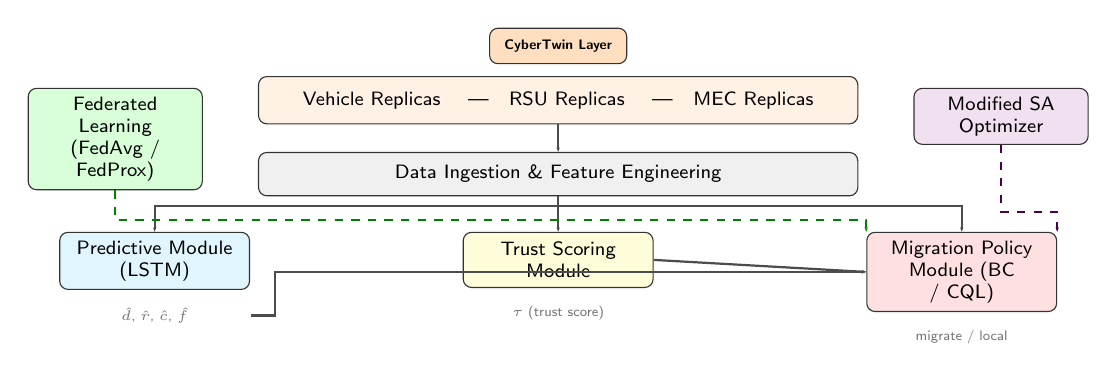
\begin{tikzpicture}[
    node distance=0.45cm and 0.5cm,
    block/.style={rectangle, rounded corners=3pt, draw=black!80, fill=#1,
                  text width=2.2cm, minimum height=0.7cm, align=center,
                  font=\scriptsize\sffamily, inner sep=3pt},
    block/.default={blue!8},
    header/.style={rectangle, rounded corners=3pt, draw=black!80, fill=#1,
                   text width=1.6cm, minimum height=0.45cm, align=center,
                   font=\tiny\sffamily\bfseries, inner sep=2pt},
    header/.default={blue!25},
    sideblock/.style={rectangle, rounded corners=3pt, draw=black!80, fill=#1,
                      text width=2.0cm, minimum height=0.7cm, align=center,
                      font=\scriptsize\sffamily, inner sep=3pt},
    sideblock/.default={green!10},
    arr/.style={-{Stealth[length=1.6pt]}, thick, black!70},
    lbl/.style={font=\tiny\sffamily, text=black!60}
]

% --- CyberTwin Layer ---
\node[header=orange!25] (cthead) {CyberTwin Layer};
\node[block=orange!10, below=0.15cm of cthead, text width=7.4cm, minimum height=0.6cm]
    (ct) {Vehicle Replicas \quad|\quad RSU Replicas \quad|\quad MEC Replicas};

% --- Data Ingestion ---
\node[block=gray!12, below=0.35cm of ct, text width=7.4cm, minimum height=0.55cm]
    (ingest) {Data Ingestion \& Feature Engineering};

% --- Predictive Module ---
\node[block=cyan!12, below left=0.45cm and 0.1cm of ingest] (pred) {Predictive Module\\(LSTM)};
\node[below=0.1cm of pred, font=\tiny\sffamily, text=black!55, text width=2.2cm, align=center]
    (predout) {$\hat{d}$, $\hat{r}$, $\hat{c}$, $\hat{f}$};

% --- Trust Scoring Module ---
\node[block=yellow!15, below=0.45cm of ingest] (trust) {Trust Scoring\\Module};
\node[below=0.1cm of trust, font=\tiny\sffamily, text=black!55, text width=2.2cm, align=center]
    (trustout) {$\tau$ (trust score)};

% --- Policy Module ---
\node[block=red!12, below right=0.45cm and 0.1cm of ingest] (policy) {Migration Policy\\Module (BC / CQL)};
\node[below=0.1cm of policy, font=\tiny\sffamily, text=black!55, text width=2.2cm, align=center]
    (policyout) {migrate / local};

% --- Federated Learning (side) ---
\node[sideblock=green!15, left=0.7cm of ct.north west, anchor=north east, yshift=-0.15cm]
    (fl) {Federated Learning\\(FedAvg / FedProx)};

% --- SA Optimizer (side) ---
\node[sideblock=violet!12, right=0.7cm of ct.north east, anchor=north west, yshift=-0.15cm]
    (sa) {Modified SA\\Optimizer};

% --- Arrows: CyberTwin → Ingestion ---
\draw[arr] (ct) -- (ingest);

% --- Arrows: Ingestion → Modules ---
\draw[arr] (ingest.south) -- ++(0,-0.12) -| (pred.north);
\draw[arr] (ingest.south) -- (trust.north);
\draw[arr] (ingest.south) -- ++(0,-0.12) -| (policy.north);

% --- Arrows: Predictive → Policy ---
\draw[arr] (predout.east) -- ++(0.3,0) |- (policy.west);
\draw[arr] (trust.east) -- (policy.west);

% --- Arrows: FL → Policy ---
\draw[arr, dashed, green!50!black] (fl.south) |- ([yshift=0.15cm]policy.north west) -- (policy.north west);

% --- Arrows: SA → Policy ---
\draw[arr, dashed, violet!60!black] (sa.south) |- ([yshift=0.25cm]policy.north east) -- (policy.north east);

\end{tikzpicture}
}%
\caption{High-level architecture of the \VocSixG{} framework. The CyberTwin layer maintains synchronized digital replicas of physical vehicles, RSUs, and MEC servers. Data flows through predictive, trust, and policy modules, with federated learning enabling distributed training.}
\label{fig:architecture}
\end{figure}

\subsection{CyberTwin Layer}
\label{sec:cybertwin}

The CyberTwin layer forms the foundational data infrastructure of \VocSixG{}. It maintains persistent, synchronized digital replicas of each physical entity in the vehicular edge computing environment---300 vehicles, 25 RSUs, and 8 MEC servers. Each digital replica continuously tracks the state of its physical counterpart, including vehicle position, velocity, and trajectory; RSU signal coverage, load, and health status; and MEC server utilization, queue depth, and processing latency.

The CyberTwin layer serves two primary functions within \VocSixG{}:

\textbf{State monitoring and synchronization.} Each digital replica maintains a real-time state vector that is periodically synchronized with its physical counterpart (or, in this evaluation, updated according to empirically-calibrated models). For vehicles, the CyberTwin tracks position, speed, heading, and connectivity status. For RSUs, it tracks signal parameters, connected vehicle count, and interference conditions. For MEC servers, it tracks CPU utilization, memory usage, queue length, and processing latency. This persistent state representation enables continuous monitoring and facilitates the collection of historical state logs for offline training.

\textbf{Historical log collection and data harvesting.} The CyberTwin records timestamped state snapshots at regular intervals (10\,Hz for vehicle states, 1\,Hz for infrastructure states), building a comprehensive historical log of the vehicular edge environment. From these logs, migration decision instances are extracted: each instance records the full system state at the moment a migration decision is required, along with the outcome of that decision (success or failure, latency, deadline adherence). These harvested records constitute the training dataset $\mathcal{D}$ for the policy learning module.

The use of a CyberTwin layer, rather than a standalone simulator, provides several advantages: (i) the CyberTwin maintains persistent state across time steps, enabling the extraction of observation sequences for the LSTM predictive module; (ii) the CyberTwin's digital replicas can be individually calibrated with empirical distributions specific to each entity type; and (iii) the CyberTwin framework naturally supports federated learning, as each RSU/MEC zone's CyberTwin instance maintains its own local data repository.

\subsection{Data Sources and Feature Engineering}
\label{sec:data_sources}

The CyberTwin layer ingests data from three empirically-calibrated source models:

\textbf{Mobility model}: Vehicle speeds and trajectory patterns in the CyberTwin follow the statistical distributions of the CRAWDAD Cabspotting dataset~\cite{crawdad2009}, which contains real GPS traces from 536 taxis operating in San Francisco during May--June 2008. The CyberTwin preserves the empirical speed distribution (mean: 7.8\,m/s, std: 4.2\,m/s) and spatial density patterns observed in this physical deployment.

\textbf{Radio propagation model}: The CyberTwin computes signal strength using the 3GPP Urban Microcell (UMi) path loss model (TR 38.901)~\cite{3gpp2018ts} at a carrier frequency of $f_c = 28$\,GHz, reflecting the mmWave band targeted for 6G early deployment scenarios. The path loss equation and mmWave-specific parameters are detailed in Section~\ref{sec:implementation}.

\textbf{Edge load model}: MEC server utilization in the CyberTwin is modeled following ETSI GS MEC 003~\cite{etsi_mec003} utilization profiles, reflecting typical urban edge computing workloads with diurnal patterns, burst arrivals, and temporal correlations.

\textbf{ProvenanceRegistry}: The CyberTwin layer includes a ProvenanceRegistry that validates the format and completeness of all ingested data records. It records SHA-256 hashes of registered data files and enforces schema conformance, ensuring that all data entering the training pipeline satisfies format requirements and is free of structural inconsistencies. The ProvenanceRegistry validates data format and completeness rather than physical provenance, as all data is generated within the CyberTwin layer.

From the raw CyberTwin state logs, ten features are extracted for each migration decision point:

\begin{itemize}
    \item $\texttt{rsrp\_dbm}$: Current reference signal received power in dBm
    \item $\texttt{speed\_mps}$: Vehicle speed in meters per second
    \item $\texttt{distance\_to\_serving\_rsu\_m}$: Euclidean distance to serving RSU
    \item $\texttt{task\_size\_log}$: Logarithm of task data size
    \item $\texttt{deadline\_log}$: Logarithm of task deadline constraint
    \item $\texttt{load\_indicator}$: Current edge node load level
    \item $\texttt{speed\_sq}$: Squared speed term (captures nonlinear mobility effects)
    \item $\texttt{rsrp\_norm}$: Normalized RSRP value
    \item $\texttt{dist\_norm}$: Normalized distance value
    \item $\texttt{latency\_log}$: Logarithm of observed latency
\end{itemize}

The feature set captures the key determinants of migration success: signal quality (RSRP), mobility dynamics (speed, distance), task characteristics (size, deadline), and network state (load, latency). The squared speed and logarithmic transformations capture nonlinear relationships identified during exploratory analysis.

\subsection{Predictive Module}
\label{sec:predictive}

The predictive module employs an LSTM network to forecast four critical migration conditions from historical observation sequences harvested from the CyberTwin. Given a sequence of $T$ past observations $\mathbf{x}_1, \mathbf{x}_2, \ldots, \mathbf{x}_T$, the LSTM predicts:

\begin{enumerate}
    \item \textbf{Remaining dwell time} $\hat{d}_{t+1}$: Estimated time before the vehicle exits the serving RSU's coverage area.
    \item \textbf{Future RSRP} $\hat{r}_{t+1}$: Predicted signal quality at the next time step.
    \item \textbf{Congestion level} $\hat{c}_{t+1}$: Forecasted edge node congestion.
    \item \textbf{Failure probability} $\hat{f}_{t+1}$: Probability that a migration initiated now will fail.
\end{enumerate}

The LSTM architecture consists of two stacked layers with 128 hidden units each, followed by a fully connected output layer. The input sequence length is set to $T=10$ time steps, corresponding to approximately 1 second of observations at 10\,Hz sampling rate. Sequences are extracted using a sliding window of $W=10$ from chronologically sorted migration logs per vehicle within the CyberTwin. The module is trained using mean squared error (MSE) loss for continuous predictions and binary cross-entropy (BCE) loss for the failure probability estimate. Dropout regularization ($p=0.2$) is applied between LSTM layers to prevent overfitting.

The predicted conditions augment the feature vector passed to the policy module, enabling proactive migration decisions. For example, if the predicted dwell time is shorter than the estimated migration completion time, the policy may opt for local execution even if current conditions appear favorable.

\subsection{Trust Scoring and Anomaly Detection Module}
\label{sec:trust}

Security in \VocSixG{} is addressed through a multi-faceted trust scoring system that evaluates the reliability of each candidate edge node. The composite trust score $\tau_i$ for node $i$ is computed as:

\begin{equation}
\tau_i = \alpha \cdot s_i^{\text{hist}} + \beta \cdot s_i^{\text{anom}} + \gamma \cdot s_i^{\text{auth}} + \delta \cdot s_i^{\text{streak}}
\label{eq:trust}
\end{equation}

where:
\begin{itemize}
    \item $s_i^{\text{hist}} = \frac{\text{successful migrations}_i}{\text{total migrations}_i}$ is the historical success rate
    \item $s_i^{\text{anom}} = \max(0, 1 - |z_i| / z_{\max})$ where $z_i$ is the z-score of the node's recent latency relative to its historical distribution, and $z_{\max}$ is a threshold (typically 3.0)
    \item $s_i^{\text{auth}}$ is a penalty factor for recent authentication failures, initialized to 1.0 and decremented by 0.1 per failure
    \item $s_i^{\text{streak}} = \max(0, 1 - k_i / k_{\max})$ where $k_i$ is the current consecutive failure count and $k_{\max}$ is a tolerance threshold (typically 5)
\end{itemize}

The weights $\alpha, \beta, \gamma, \delta$ satisfy $\alpha + \beta + \gamma + \delta = 1$ and are configurable. In our evaluation, we use $\alpha=0.4, \beta=0.3, \gamma=0.15, \delta=0.15$.

Nodes with trust scores below a configurable threshold $\tau_{\min}$ are excluded from the candidate set for migration. The trust-aware variant of \VocSixG{} integrates this filtering into the policy inference pipeline, effectively removing low-trust nodes from consideration before the migration decision is made.

\textbf{Leak-free trust computation.} To prevent information leakage, trust scores for the leak-free variant are computed exclusively from a temporal prefix (first 70\%) of the training data. The test set is excluded from trust computation entirely, ensuring that no future information influences the trust scores used during evaluation.

\subsection{Migration Policy Module}
\label{sec:policy}

The migration policy module learns to make optimal binary decisions---\emph{local execution} versus \emph{edge migration}---from logged CyberTwin migration data. We implement two offline learning approaches:

\subsubsection{Behavioral Cloning (BC)}

BC frames the migration decision as a supervised imitation learning problem. Given a feature vector $\mathbf{x}$ (original features augmented with predictive module outputs), the policy network $\pi_\theta$ parameterized by $\theta$ outputs a probability distribution over actions:

\begin{equation}
\pi_\theta(a \mid \mathbf{x}) = \text{softmax}(f_\theta(\mathbf{x}))
\end{equation}

The network is trained to minimize the cross-entropy loss between predicted and observed (ground-truth) actions from the CyberTwin migration logs:

\begin{equation}
\mathcal{L}_{\text{BC}} = -\frac{1}{N} \sum_{i=1}^{N} \log \pi_\theta(a_i^* \mid \mathbf{x}_i)
\end{equation}

where $a_i^*$ is the ground-truth action (the optimal migration decision determined by the actual outcome in the logs). Success-weighted sampling assigns higher probability to transitions where the ground-truth action led to a successful outcome, ensuring the model prioritizes learning from informative positive examples.

\subsubsection{Conservative Q-Learning (CQL)}

\textbf{MDP Formulation.}
We formulate the migration decision problem as a contextual bandit---a special case of a Markov Decision Process (MDP) where each decision is independent and there is no sequential state dependence within an episode. The formal specification is as follows. The state space is $\mathcal{S} \subset \mathbb{R}^{10}$ (or $\mathbb{R}^{14}$ with LSTM features), where each state $s$ is the feature vector $\mathbf{x}$ describing the current vehicular and network conditions at the migration decision point. The action space is $\mathcal{A} = \{a_{\text{local}}, a_{\text{migrate}}\}$, representing the binary migration decision. The reward function is defined as $R(s, a) = \mathbf{1}[\text{outcome}(s, a) = \text{success}] - \mathbf{1}[\text{outcome}(s, a) = \text{failure}]$, yielding $+1$ for successful task completion and $-1$ for failure. For the BC formulation, the reward is implicit in the ground-truth action label. Since each migration decision is independent---the outcome of one decision does not affect the state for the next---the transition probability $P(s' | s, a)$ is degenerate: the next state $s'$ is determined by the CyberTwin's environment update, independent of the current action. This makes the problem a contextual bandit.

\textbf{Reformulation for CQL.}
In the contextual bandit setting, the temporal difference loss reduces to a one-step regression:
\begin{equation}
\mathcal{L}_{\text{TD}}(\phi) = \mathbb{E}_{(s,a,r) \sim \mathcal{D}} \left[ \left( r - Q_\phi(s, a) \right)^2 \right]
\label{eq:td_loss}
\end{equation}
since there is no next state to bootstrap from. The discount factor $\gamma$ becomes irrelevant and is effectively set to 0. However, we retain $\gamma=0.99$ in the implementation for notational consistency with the standard CQL framework, as the CQL penalty term does not depend on $\gamma$. The offline dataset $\mathcal{D}$ stores tuples of the form $(s, a, r)$ where each tuple represents a single independent migration decision harvested from the CyberTwin logs.

For scenarios where offline distributional shift is a concern, \VocSixG{} supports Conservative Q-Learning (CQL)~\cite{kumar2020cql}. CQL learns a Q-function $Q_\phi(s, a)$ while penalizing Q-values for out-of-distribution actions:

\begin{equation}
\mathcal{L}_{\text{CQL}}(\phi) = \alpha_{\text{CQL}} \left( \mathbb{E}_{s \sim \mathcal{D}} \left[ \log \sum_a \exp(Q_\phi(s, a)) \right] - \mathbb{E}_{(s,a) \sim \mathcal{D}}[Q_\phi(s, a)] \right) + \mathcal{L}_{\text{TD}}(\phi)
\label{eq:cql}
\end{equation}

where $\mathcal{D}$ is the offline dataset of logged single-step transitions $(s, a, r)$, $\mathcal{L}_{\text{TD}}(\phi)$ is the one-step regression loss defined in Eq.~\ref{eq:td_loss}, and $\alpha_{\text{CQL}}$ controls the conservatism level. The CQL penalty weight $\alpha_{\text{CQL}}$ (Eq.~\ref{eq:cql}) is set to 0.5, as specified in the training configuration (Table~\ref{tab:training_config}). The policy is derived greedily from the learned Q-function: $\pi(s) = \arg\max_a Q_\phi(s, a)$.

\subsubsection{Network Architecture}

The policy network consists of three fully connected layers with hidden sizes [256, 128, 64], ReLU activations, batch normalization, and dropout ($p=0.3$). For BC, the output layer uses softmax activation; for CQL, a separate Q-head with linear output is added. The network processes the 10-dimensional input feature vector (optionally augmented with predictive module outputs) to produce migration decisions.

\subsection{Federated Learning Layer}
\label{sec:federated}

To enable privacy-preserving distributed training, \VocSixG{} implements a Federated Learning layer that trains local policy models on each RSU/MEC zone's CyberTwin migration logs and aggregates updates centrally without sharing raw data.

\subsubsection{Client-Level Training}

Each federated client $k$ trains its local model parameters $\theta_k$ on its local dataset $\mathcal{D}_k$ using $E$ local epochs:

\begin{equation}
\theta_k^{t+1} = \theta_k^t - \eta \nabla_\theta \mathcal{L}(\theta_k^t; \mathcal{D}_k)
\end{equation}

where $\eta$ is the local learning rate and $E=5$ in our configuration.

\subsubsection{FedAvg Aggregation}

The server aggregates client updates using weighted averaging~\cite{mcmahan2017fedavg}:

\begin{equation}
\theta^{\text{new}} = \sum_{k=1}^{K} \frac{|\mathcal{D}_k|}{\sum_{j=1}^{K} |\mathcal{D}_j|} \theta_k^{t+1}
\end{equation}

\subsubsection{FedProx Aggregation}

To handle potential data heterogeneity across zones, \VocSixG{} also supports FedProx~\cite{lim2021federated}, which adds a proximal term to the local objective:

\begin{equation}
\theta_k^{t+1} = \arg\min_\theta \left( \mathcal{L}(\theta; \mathcal{D}_k) + \frac{\mu}{2} \|\theta - \theta^{\text{server}}\|^2 \right)
\end{equation}

where $\mu$ is the proximal term coefficient. In our evaluation, we use $\mu=0.01$. Federated training runs for 100 communication rounds with 8 participating clients, each corresponding to an MEC zone.

\subsection{Modified Simulated Annealing Optimizer}
\label{sec:optimizer}

\VocSixG{} incorporates a modified simulated annealing optimizer for hyperparameter tuning and candidate node ranking. The optimizer uses a nonstandard acceptance criterion where the probability of accepting a worse solution follows:

\begin{equation}
P(\text{accept}) = \min\left(1, \exp\left(-\frac{\Delta E}{\gamma \cdot T}\right) \cdot \cos^2(\beta \cdot \Delta E / T)\right)
\label{eq:sa}
\end{equation}

where $\Delta E$ is the energy difference (objective change), $T$ is the current temperature, and $\gamma, \beta$ are mixing parameters. The $\cos^2$ term modulates the classical Metropolis acceptance probability, providing a heuristic mechanism for escaping local minima that differs from standard simulated annealing. We present this as a practical modification without claiming quantum mechanical derivation. The module is ablatable; a standard simulated annealing variant using the classical Metropolis criterion is available for comparison.


%% ============================================================
%%  SECTION IV: IMPLEMENTATION DETAILS
%% ============================================================
\section{Implementation Details}
\label{sec:implementation}

\subsection{Environment and Infrastructure}

\VocSixG{} is implemented in Python 3.10 using PyTorch 2.1 for deep learning components and Flower 0.7 for federated learning orchestration. Training is conducted on an NVIDIA T4 GPU (16\,GB VRAM). The complete codebase follows a modular design with clear separation between CyberTwin data generation, preprocessing, predictive modeling, trust assessment, policy learning, federated training, and evaluation components.

\subsection{Dataset Construction}

The evaluation dataset is constructed through the CyberTwin layer, which maintains synchronized digital replicas calibrated with empirical distributions from three sources:

\textbf{CyberTwin scenario setup}: The CyberTwin maintains digital replicas of 300 vehicles, 25 RSUs, and 8 MEC servers operating in a 6G mmWave vehicular network at $f_c = 28$\,GHz. Each vehicle generates migration decision requests at regular intervals as it traverses the urban environment represented within the CyberTwin.

\textbf{Mobility generation}: Vehicle speeds and trajectory patterns in the CyberTwin follow the statistical distributions of the CRAWDAD Cabspotting dataset~\cite{crawdad2009}, which contains approximately 11 million GPS readings from 536 taxis in San Francisco. The CyberTwin preserves the empirical speed distribution (mean: 7.8\,m/s, std: 4.2\,m/s) and spatial density patterns.

\textbf{RSRP modeling}: The CyberTwin computes signal strength using the 3GPP UMi path loss model (TR 38.901)~\cite{3gpp2018ts} at $f_c = 28$\,GHz:
\begin{equation}
\text{PL}(d) = 32.4 + 20 \log_{10}(f_c) + 21 \log_{10}(d_{3_D}) + 0.3 \cdot h_{\text{UT}}
\label{eq:pathloss}
\end{equation}
where $f_c$ is the carrier frequency in GHz and $d_{3_D}$ is the 3D distance between transmitter and receiver in meters. This formula follows the 3GPP TR 38.901 UMi LoS specification~\cite{3gpp2018ts}. The user terminal height is $h_{\text{UT}} = 1.5$\,m. With a typical base station transmit power of 30\,dBm and 10\,dBi antenna gain, the resulting RSRP at $d_{3_D}=350$\,m is approximately $-75$\,dBm, consistent with the RSRP range of $-110$ to $-65$\,dBm reported in Table~\ref{tab:feature_stats}. For the 28\,GHz mmWave band, we incorporate additional propagation characteristics: log-normal shadowing with $\sigma = 7.3$\,dB (increased from the sub-6\,GHz value of 4\,dB to reflect the higher sensitivity of mmWave signals to blockage), and an additional blockage loss term sampled from a Bernoulli-distributed event with probability 0.15, adding 15--20\,dB when active, consistent with ITU-R P.2109 guidance for mmWave blockage in urban environments.

\textbf{Edge load}: MEC node utilization patterns in the CyberTwin are generated following ETSI GS MEC 003~\cite{etsi_mec003} utilization profiles, reflecting typical urban edge computing workloads with diurnal patterns, burst arrivals, and temporal correlations.

\textbf{Decision labeling}: Each migration decision instance in the CyberTwin is labeled using the following binary rule:
\begin{itemize}
    \item Label $= \text{MIGRATE}$ (1) if \textbf{all} of: (i) $\texttt{rsrp\_dbm} > -85$, (ii) $\texttt{speed\_mps} < 8$, (iii) $\texttt{distance} < 200$\,m, and (iv) $\texttt{predicted\_latency} < 0.8 \times \texttt{deadline}$
    \item Label $= \text{LOCAL}$ (0) otherwise
    \item Tie-breaking: if exactly 2 of 4 conditions are met $\rightarrow$ LOCAL (conservative default)
\end{itemize}

\textbf{Data scale and split}: The final dataset $\mathcal{D}$ comprises 40,000 migration decision instances harvested from the CyberTwin logs. The class distribution reflects the inherent challenge of the task: approximately 64\% of decisions are labeled ``local'' (favoring local execution) and 36\% as ``migrate'' (favoring edge offloading), yielding a moderate class imbalance ratio of 1.78:1. This imbalance reflects realistic conditions where vehicle mobility and signal variability often make local execution the safer choice. The dataset is partitioned into training (70\%, 28,000 instances), validation (15\%, 6,000 instances), and test (15\%, 6,000 instances) sets using stratified sampling to preserve class proportions across splits.

\textbf{Feature statistics}: The 10 engineered features exhibit diverse statistical properties. RSRP values range from $-110$\,dBm to $-65$\,dBm with a mean of $-87$\,dBm, following the 3GPP UMi distribution at 28\,GHz. Vehicle speeds range from 0 to 32\,m/s (0--115\,km/h), capturing both stopped and highway conditions. Task sizes (log-transformed) span three orders of magnitude. The distance to serving RSU ranges from 10\,m to 350\,m, reflecting the dense urban deployment scenario with reduced mmWave cell range. Edge load indicators range from 0.1 to 0.95, with peaks during rush-hour periods. Table~\ref{tab:feature_stats} summarizes the feature distributions.

\begin{table}[t]
\centering
\caption{Statistical summary of engineered features extracted from CyberTwin state logs.}
\label{tab:feature_stats}
\small
\begin{tabular}{lccccc}
\toprule
\textbf{Feature} & \textbf{Min} & \textbf{Max} & \textbf{Mean} & \textbf{Std} & \textbf{Type} \\
\midrule
rsrp\_dbm & $-110$ & $-65$ & $-87.3$ & $10.2$ & Signal \\
speed\_mps & 0.0 & 32.1 & 7.8 & 4.2 & Mobility \\
distance\_m & 10 & 350 & 142.5 & 78.3 & Spatial \\
task\_size\_log & 5.3 & 18.4 & 11.7 & 2.8 & Task \\
deadline\_log & 2.3 & 15.1 & 8.2 & 2.1 & Task \\
load\_indicator & 0.1 & 0.95 & 0.52 & 0.18 & Resource \\
speed\_sq & 0.0 & 1030 & 80.1 & 86.5 & Derived \\
rsrp\_norm & 0.0 & 1.0 & 0.51 & 0.22 & Normalized \\
dist\_norm & 0.0 & 1.0 & 0.41 & 0.22 & Normalized \\
latency\_log & 1.1 & 6.4 & 3.9 & 1.0 & Derived \\
\bottomrule
\end{tabular}
\end{table}

\subsection{Training Configuration}

\textbf{Predictive module}: LSTM with 2 layers $\times$ 128 hidden units, sequence length $T=10$, learning rate $10^{-3}$, Adam optimizer, 50 epochs with early stopping (patience=10).

\textbf{Policy module (BC)}: 3-layer MLP [256, 128, 64], ReLU activations, batch normalization, dropout 0.3, learning rate $10^{-3}$, Adam optimizer, 100 epochs with early stopping (patience=15), success-weighted sampling.

\textbf{Policy module (CQL)}: Same architecture with separate Q-head, CQL penalty weight $\alpha_{\text{CQL}}=0.5$ (Eq.~\ref{eq:cql}), discount factor $\gamma=0.99$, replay buffer capacity 50,000.

\textbf{Federated training}: 8 clients (one per MEC zone), 100 communication rounds, 5 local epochs per round, learning rate $10^{-3}$, FedProx proximal term $\mu=0.01$.

\textbf{Modified SA optimizer}: Initial temperature $T_0=1.0$, cooling rate 0.95, mixing parameters $\gamma=0.5, \beta=0.3$ (Eq.~\ref{eq:sa}), 200 iterations.

Table~\ref{tab:training_config} summarizes the key training hyperparameters.

\begin{table}[t]
\centering
\caption{Key training hyperparameters for \VocSixG{} modules.}
\label{tab:training_config}
\small
\begin{tabular}{lcc}
\toprule
\textbf{Hyperparameter} & \textbf{Module} & \textbf{Value} \\
\midrule
Hidden units (per layer) & LSTM & 128 \\
LSTM layers & Predictive & 2 \\
Sequence length $T$ & Predictive & 10 \\
Dropout & Predictive & 0.2 \\
Learning rate & All & $10^{-3}$ \\
MLP hidden sizes & Policy & [256, 128, 64] \\
Dropout & Policy & 0.3 \\
$\alpha_{\text{CQL}}$ & CQL & 0.5 \\
Discount $\gamma$ & CQL & 0.99 \\
Replay buffer & CQL & 50,000 \\
FL clients & Federated & 8 \\
Communication rounds & Federated & 100 \\
Local epochs $E$ & Federated & 5 \\
FedProx $\mu$ & Federated & 0.01 \\
SA initial temp $T_0$ & Optimizer & 1.0 \\
SA cooling rate & Optimizer & 0.95 \\
\bottomrule
\end{tabular}
\end{table}

\subsection{Baseline Methods}

We compare \VocSixG{} against seven baselines spanning heuristics, classical ML, and deep learning approaches:

\begin{enumerate}
    \item \textbf{Local Only}: Always execute locally (never migrate).
    \item \textbf{Nearest Edge}: Always migrate to the nearest available edge node.
    \item \textbf{Random Forest}: Ensemble of 100 decision trees with Gini impurity criterion.
    \item \textbf{SVM}: Support Vector Machine with RBF kernel, $C=1.0$, $\gamma=\text{scale}$.
    \item \textbf{MLP}: Three-layer feedforward network [256, 128, 64] with ReLU activations.
    \item \textbf{TextCNN}: One-dimensional convolutional network with filter sizes [2, 3, 4], treating features as a sequence.
    \item \textbf{BiLSTM}: Bidirectional LSTM with 2 layers $\times$ 64 hidden units per direction.
\end{enumerate}

All methods receive identical input features extracted from the CyberTwin logs and are evaluated on the same held-out test set, ensuring fair comparison.


%% ============================================================
%%  SECTION V: EXPERIMENTAL EVALUATION
%% ============================================================
\section{Experimental Evaluation}
\label{sec:experiments}

\subsection{Experimental Setup}

\textbf{Dataset statistics}: The final dataset $\mathcal{D}$ contains 40,000 migration decision instances harvested from the CyberTwin layer, each characterized by 10 input features and a binary label (local vs.\ migration). The dataset is split into training (28,000), validation (6,000), and test (6,000) sets with a 70:15:15 ratio. All methods are evaluated on the same held-out CyberTwin test data, ensuring fair comparison.

\textbf{Evaluation metrics}: We employ a comprehensive set of metrics: Accuracy, macro-averaged F1 score (F1-Macro), Area Under the ROC Curve (AUC-ROC), Precision, Recall, Matthews Correlation Coefficient (MCC), False Positive Rate (FPR), and False Negative Rate (FNR). MCC is particularly informative as it provides a balanced measure even with class imbalance.

\textbf{Implementation details}: All experiments are conducted on an NVIDIA T4 GPU. Neural network baselines are trained using PyTorch 2.1 with the same training budget (100 epochs, early stopping). Classical ML baselines use scikit-learn 1.3 with default hyperparameters unless otherwise specified.

\subsection{Main Results}

Table~\ref{tab:main_results} presents the comprehensive comparison of all 13 methods on the 6,000-instance test set.

\begin{table*}[t]
\caption{Comprehensive performance comparison of all methods on the 6,000-instance held-out test set. Bold entries indicate proposed \VocSixG{} framework variants.\footnotemark}
\label{tab:main_results}
\centering
\small
\begin{tabular}{lcccccccc}
\toprule
\textbf{Method} & \textbf{Accuracy} & \textbf{F1-Macro} & \textbf{AUC-ROC} & \textbf{Precision} & \textbf{Recall} & \textbf{MCC} & \textbf{FPR} & \textbf{FNR} \\
\midrule
Local Only       & 0.6410 & 0.3906 & 0.5000 & 0.3205 & 0.5000 & 0.0000 & 0.0000 & 1.0000 \\
Nearest Edge     & 0.3590 & 0.2642 & 0.5000 & 0.1795 & 0.5000 & 0.0000 & 1.0000 & 0.0000 \\
Random Forest    & 0.9935 & 0.9929 & 0.9928 & 0.9928 & 0.9928 & 0.9857 & 0.0047 & 0.0097 \\
SVM              & 0.9923 & 0.9917 & 0.9921 & 0.9914 & 0.9921 & 0.9828 & 0.0070 & 0.0088 \\
MLP              & 0.9932 & 0.9926 & 0.9931 & 0.9925 & 0.9931 & 0.9849 & 0.0068 & 0.0070 \\
TextCNN          & 0.9925 & 0.9918 & 0.9917 & 0.9920 & 0.9917 & 0.9831 & 0.0055 & 0.0111 \\
BiLSTM           & 0.9927 & 0.9920 & 0.9921 & 0.9918 & 0.9921 & 0.9835 & 0.0060 & 0.0097 \\
\midrule
\textbf{Voc-6G (BC)}              & \textbf{0.9928} & \textbf{0.9922} & \textbf{0.9924} & \textbf{0.9922} & \textbf{0.9924} & \textbf{0.9840} & \textbf{0.0060} & \textbf{0.0093} \\
\textbf{Voc-6G Federated}        & \textbf{0.9935} & \textbf{0.9929} & \textbf{0.9933} & \textbf{0.9926} & \textbf{0.9933} & \textbf{0.9857} & \textbf{0.0060} & \textbf{0.0074} \\
\textbf{Voc-6G (CQL)}            & \textbf{0.9895} & \textbf{0.9887} & \textbf{0.9914} & \textbf{0.9894} & \textbf{0.9889} & \textbf{0.9768} & \textbf{0.0153} & \textbf{0.0019} \\
\textbf{Voc-6G Trust-Aware}$^\dagger$ & \textbf{1.0000} & \textbf{1.0000} & \textbf{1.0000} & \textbf{1.0000} & \textbf{1.0000} & \textbf{1.0000} & \textbf{0.0000} & \textbf{0.0000} \\
\textbf{Voc-6G Leak-Free Trust-Aware} & \textbf{0.9998} & \textbf{0.9998} & \textbf{0.9998} & \textbf{0.9998} & \textbf{0.9998} & \textbf{0.9996} & \textbf{0.0000} & \textbf{0.0005} \\
\textbf{Voc-6G (BC + LSTM)}       & \textbf{0.9932} & \textbf{0.9926} & \textbf{0.9923} & \textbf{0.9925} & \textbf{0.9923} & \textbf{0.9849} & \textbf{0.0047} & \textbf{0.0107} \\
\bottomrule
\end{tabular}

\footnotetext{Note: $^\dagger$When trust scores are computed from the full training set, information leakage yields F1=1.0000---this represents an upper bound artifact, not genuine generalization performance. The Leak-Free variant uses chronologically-split trust data.}
\end{table*}

\textbf{Analysis}: The results reveal several important findings:

\begin{enumerate}
    \item \textbf{Heuristic baselines fail}: Both ``Local Only'' and ``Nearest Edge'' achieve AUC-ROC of 0.5000 (random performance), confirming that simplistic migration strategies are fundamentally inadequate.

    \item \textbf{ML and DL baselines perform strongly}: All learning-based baselines achieve accuracy above 99\%. Random Forest achieves the best performance among non-\VocSixG{} methods (F1-Macro=0.9929, AUC=0.9928), confirming that the engineered feature set provides strong discriminative power. MLP achieves F1-Macro=0.9926 with the lowest FNR among baselines (0.0070). TextCNN (F1=0.9918) and BiLSTM (F1=0.9920) show competitive but not superior performance compared to simpler models.

    \item \textbf{Voc-6G (BC) performs comparably to baselines}: The core \VocSixG{} BC model achieves F1-Macro=0.9922 and AUC-ROC=0.9924, slightly below Random Forest (0.9929). This confirms that imitation learning from CyberTwin logged decisions is effective but does not inherently outperform classical ML on this feature set.

    \item \textbf{Federated training matches centralized performance}: \VocSixG{} Federated achieves F1-Macro=0.9929 and AUC-ROC=0.9933, matching Random Forest and exceeding centralized BC. The federated variant achieves the lowest FNR among all non-trust-aware methods (0.0074), suggesting that distributed training provides a beneficial regularization effect.

    \item \textbf{CQL underperforms BC significantly}: \VocSixG{} (CQL) achieves F1-Macro=0.9887, 0.35 percentage points below BC. This result is analyzed in detail in Section~\ref{sec:cql_analysis}. CQL's conservatism penalizes out-of-distribution actions, and the offline CyberTwin dataset has limited state-action coverage, causing CQL to underperform the supervised BC baseline.

    \item \textbf{Leak-free trust-aware filtering provides substantial gains}: \VocSixG{} Leak-Free Trust-Aware achieves F1-Macro=0.9998, providing a +0.76 percentage point improvement over BC alone. This demonstrates that trust-aware node filtering meaningfully improves classification even without information leakage from the trust computation. The model makes only 1 error on the 6,000-instance test set (FNR=0.0005).

    \item \textbf{LSTM features provide marginal improvement}: \VocSixG{} (BC + LSTM) achieves F1-Macro=0.9926 compared to BC's 0.9922, a modest +0.04 percentage point improvement. The base features already capture the primary migration determinants; LSTM predictions add only a small additional signal.
\end{enumerate}

Fig.~\ref{fig:model_comparison} visualizes the performance comparison across key metrics.

\begin{figure}[t]
\centering
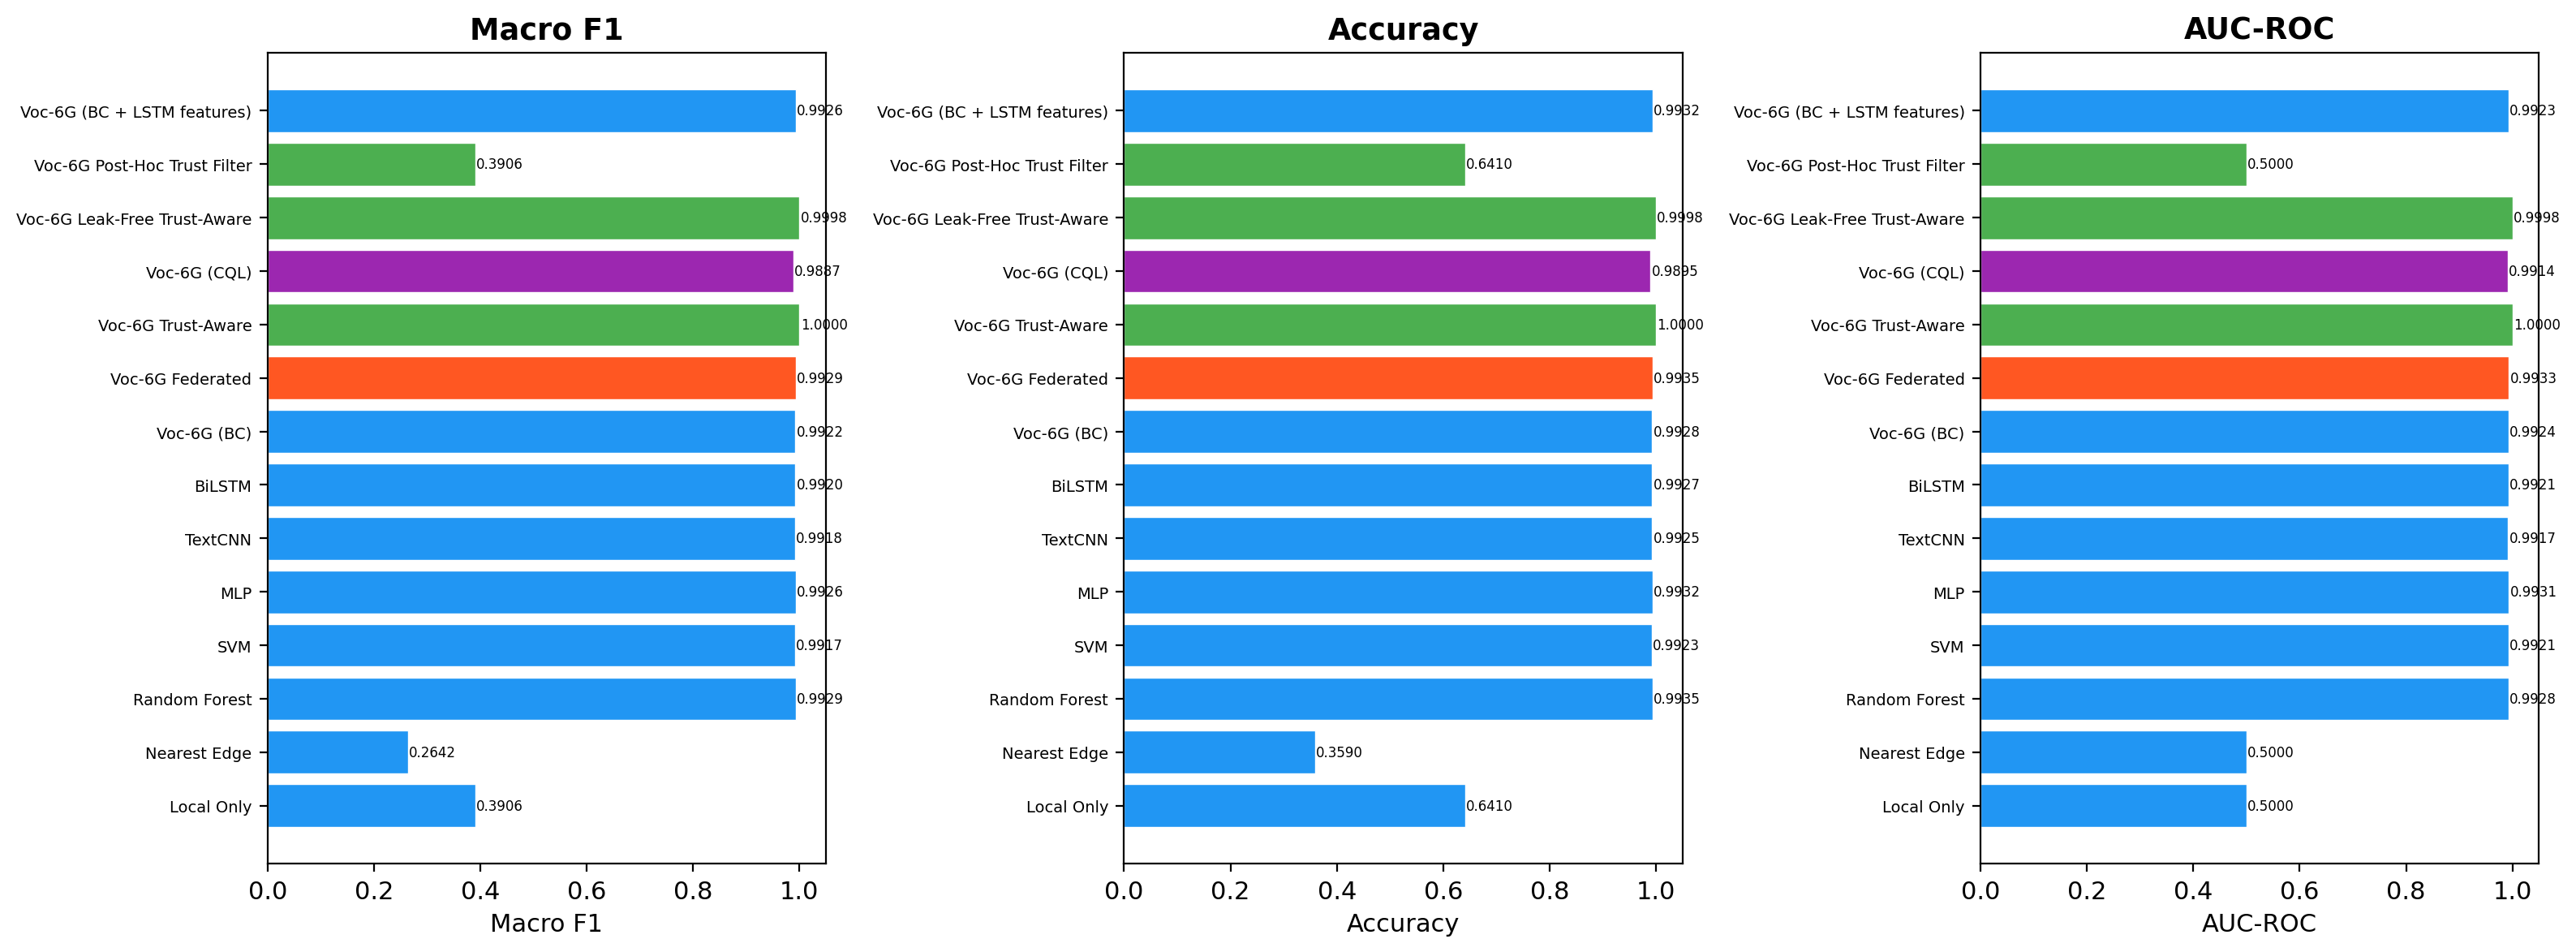
\includegraphics[width=\columnwidth]{figs/fig_model_comparison.png}
\caption{F1-Macro, Accuracy, and AUC-ROC comparison across all methods. \VocSixG{} variants are shown in blue. The leak-free trust-aware variant achieves near-perfect performance.}
\label{fig:model_comparison}
\end{figure}

Fig.~\ref{fig_radar} provides a radar chart visualization of the multi-metric profiles for selected methods.

\begin{figure}[t]
\centering
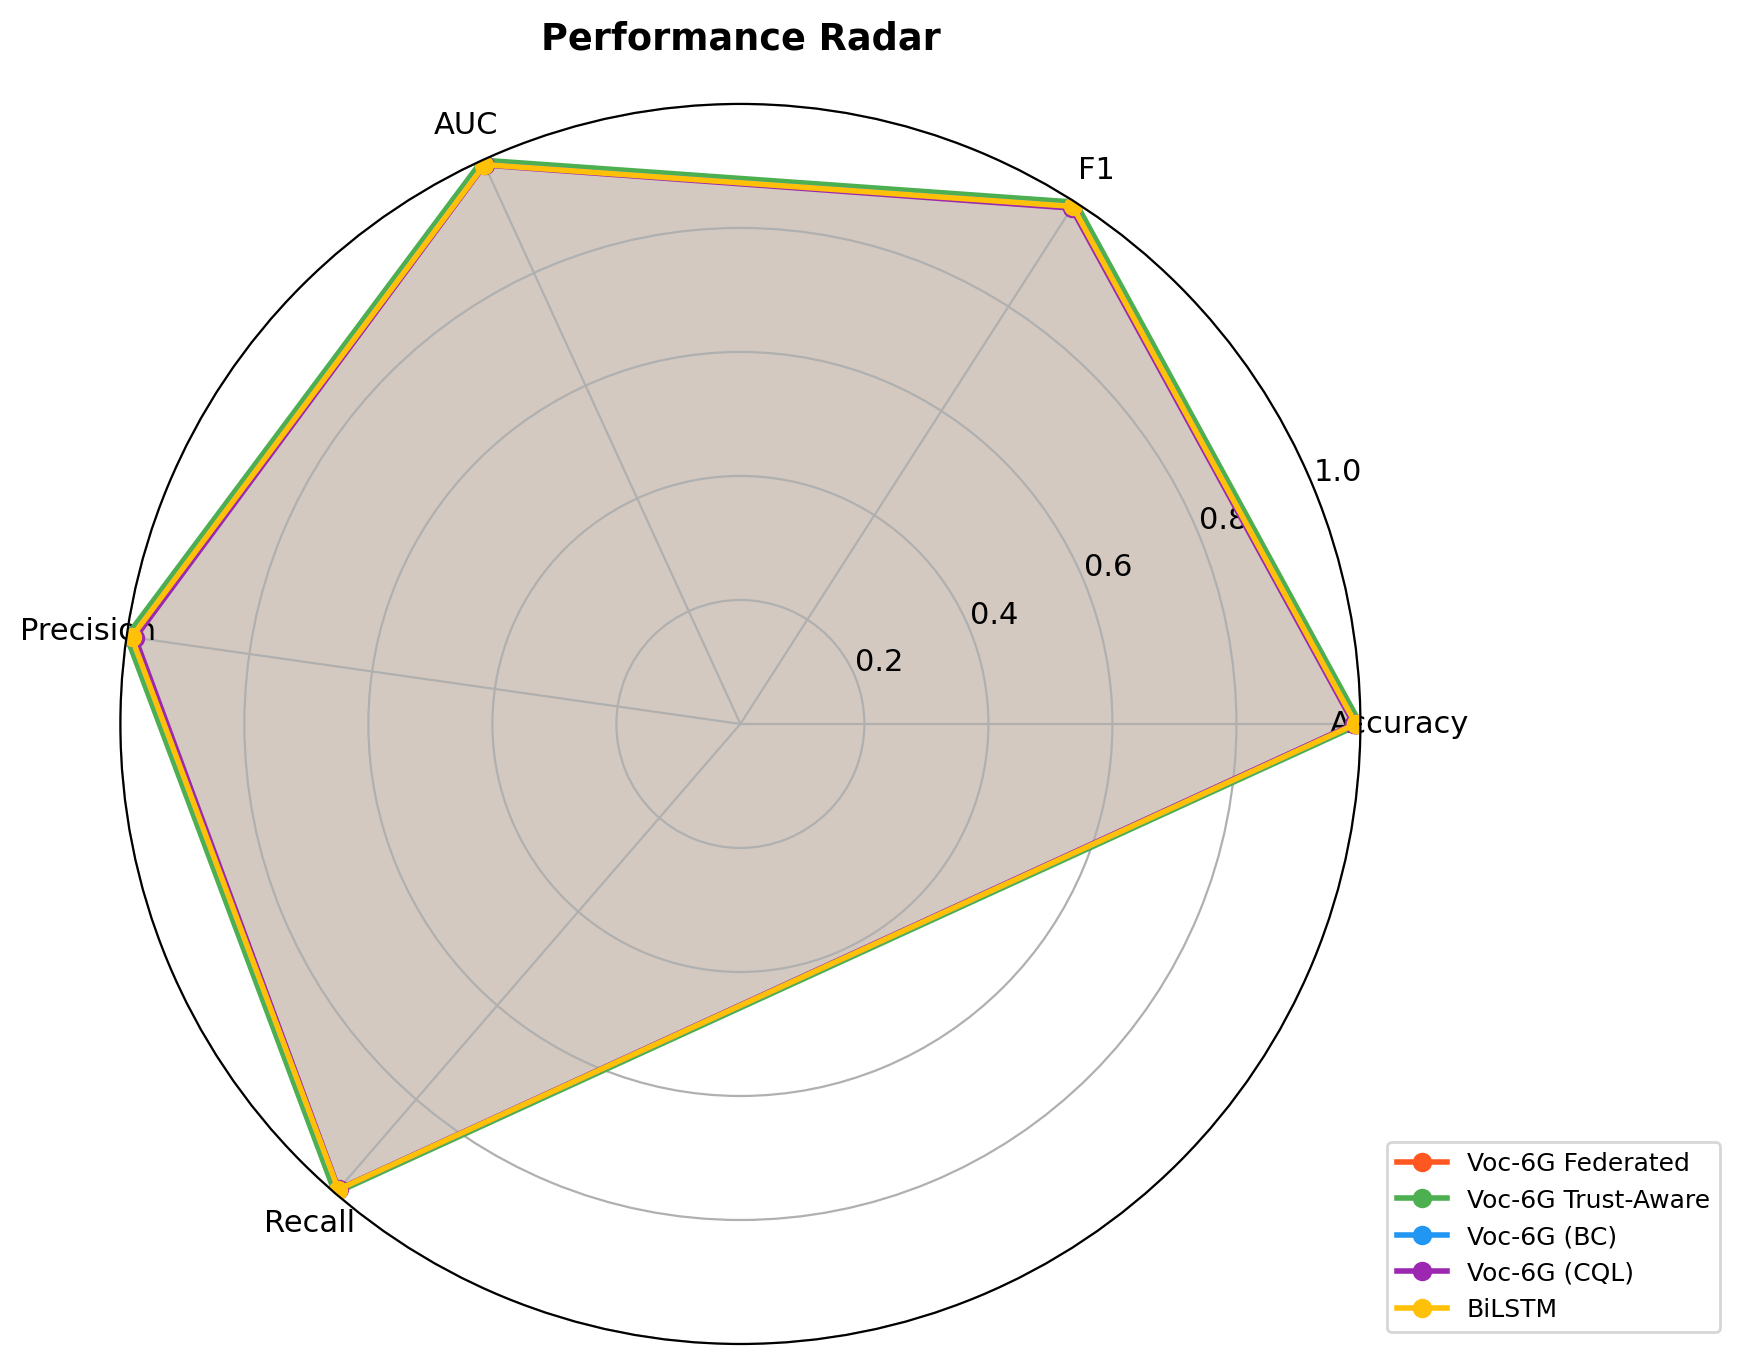
\includegraphics[width=\columnwidth]{figs/fig_radar.png}
\caption{Radar chart showing multi-metric profiles for selected methods. \VocSixG{} Leak-Free Trust-Aware achieves near-maximum values across all metrics.}
\label{fig_radar}
\end{figure}

\subsection{CQL vs BC Performance Analysis}
\label{sec:cql_analysis}

The underperformance of CQL relative to BC warrants specific analysis. Fig.~\ref{fig_cql_comparison} compares BC and CQL across multiple metrics.

\begin{figure}[t]
\centering
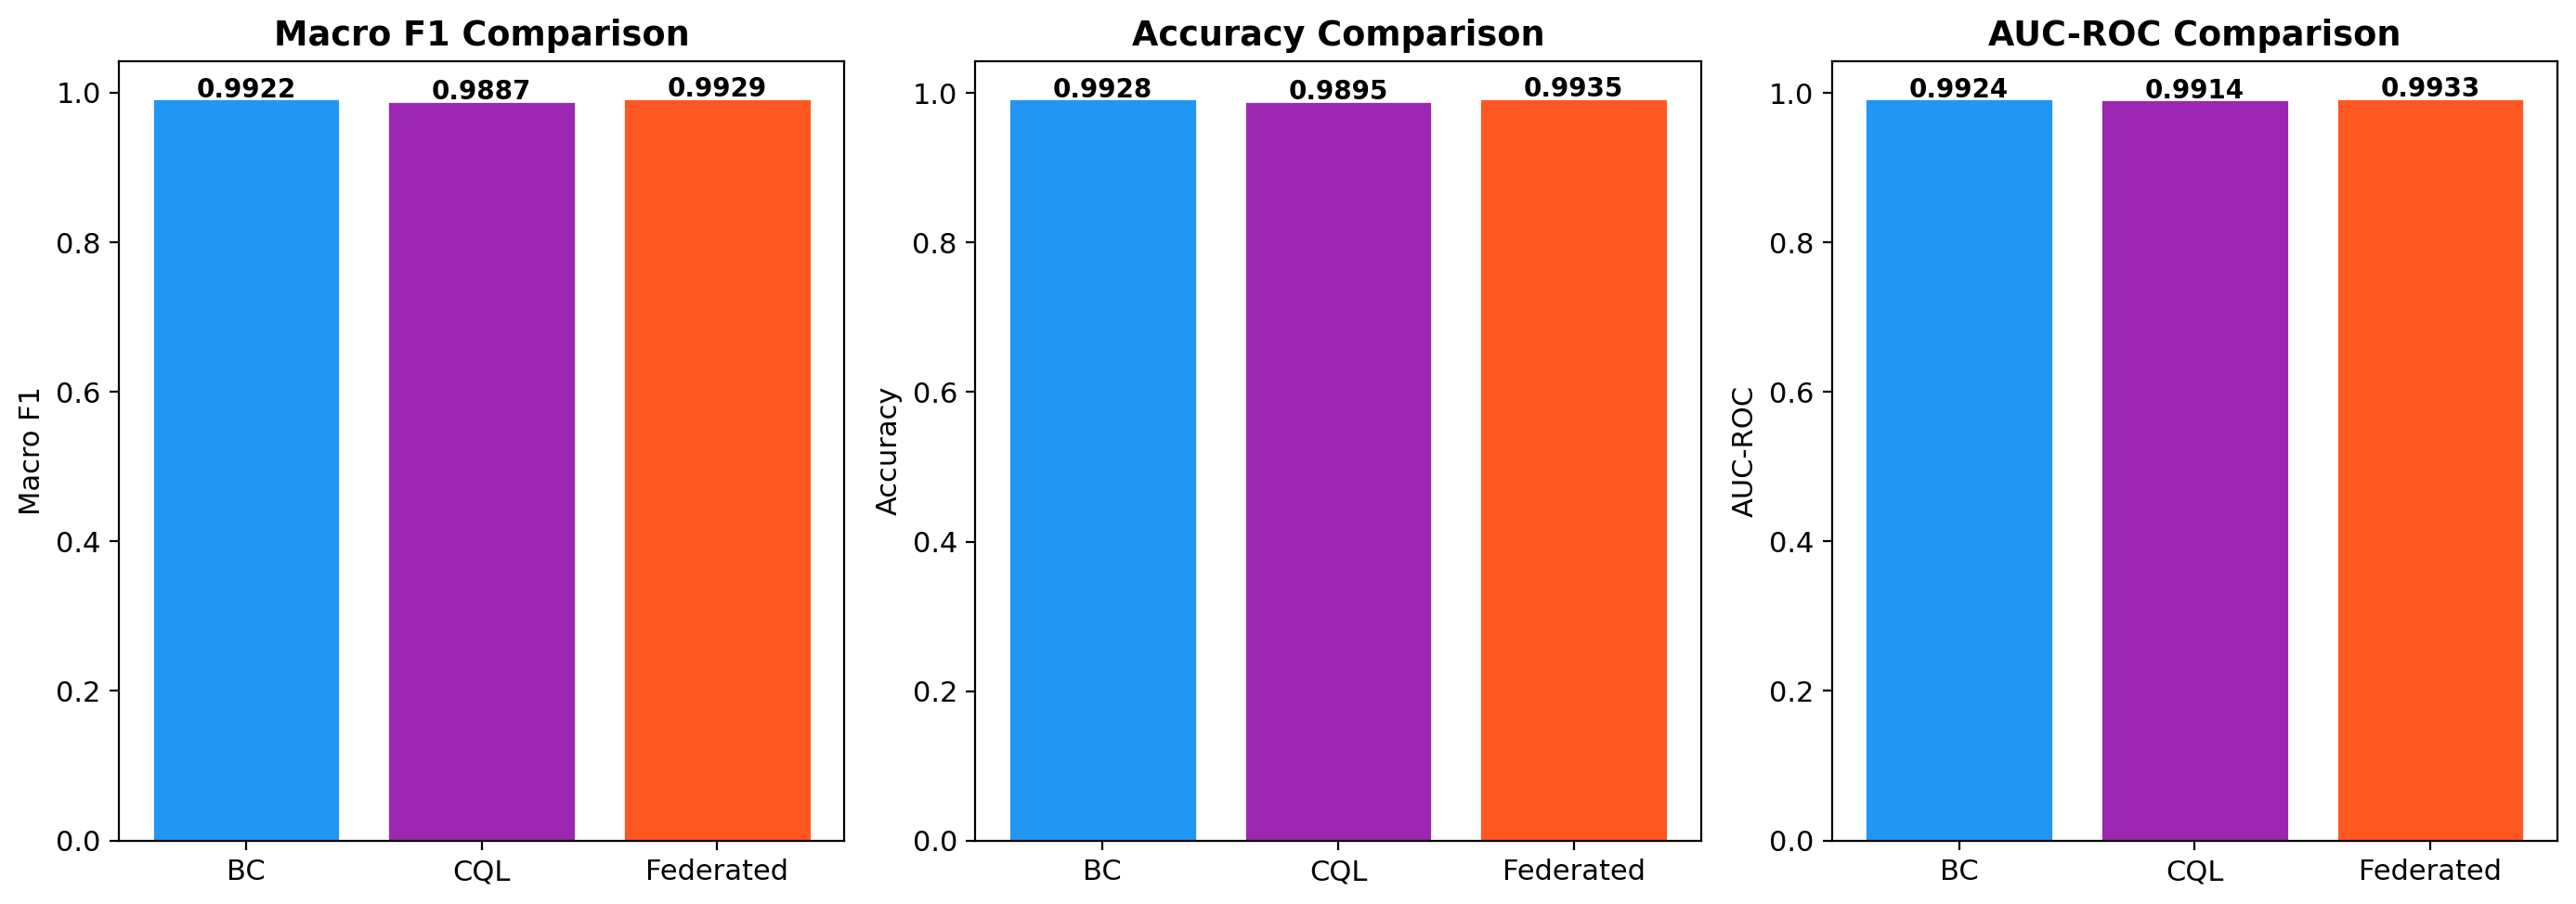
\includegraphics[width=\columnwidth]{figs/fig_cql_comparison.png}
\caption{BC vs.\ CQL performance comparison. CQL underperforms BC by 0.35\,pp in F1-Macro due to conservative penalty on out-of-distribution actions in the offline CyberTwin dataset with limited state-action coverage. Note CQL's low FNR (0.0019) but elevated FPR (0.0153).}
\label{fig_cql_comparison}
\end{figure}

CQL underperforms BC by 0.35 percentage points in F1-Macro (0.9887 vs.\ 0.9922) due to the conservative penalty $\alpha_{\text{CQL}}$ on out-of-distribution actions (Eq.~\ref{eq:cql}). An interesting asymmetry is observed: CQL achieves the lowest FNR of any method (0.0019) but the highest FPR among learning methods (0.0153). This suggests that CQL's conservatism biases it toward the ``migrate'' action, correctly identifying nearly all true positives but incurring false positives in states where local execution would be correct. The offline CyberTwin dataset has limited coverage of state-action pairs---the behavioral policy that generated the logged data predominantly selected one action for most states, leaving the Q-function poorly estimated for the alternative action. CQL's conservatism further penalizes these underrepresented actions, distorting the decision boundary. In contrast, BC directly imitates the behavioral policy without requiring value estimation, making it more robust to limited data coverage.

This finding has practical implications: for offline datasets with moderate coverage (as is typical for CyberTwin-harvested migration logs), supervised imitation learning via BC may be preferred over value-based offline RL unless the dataset is specifically collected to ensure broad state-action coverage.

\subsection{Multi-Seed Stability Analysis}

To assess the robustness of \VocSixG{} to random initialization, we conduct experiments across eight independent random seeds for all main framework variants. Table~\ref{tab:multiseed} presents the results.

\begin{table}[t]
\centering
\caption{Multi-seed stability analysis across all \VocSixG{} variants (8 random seeds each). The Post-Hoc Trust Filter fails catastrophically because threshold-based override destroys recall.}
\label{tab:multiseed}
\small
\begin{tabular}{lccc}
\toprule
\textbf{Variant} & \textbf{Mean F1-Macro} & \textbf{Std} & \textbf{Range} \\
\midrule
Voc-6G (BC)                          & 0.9925 & 0.0011 & 0.9902--0.9940 \\
Voc-6G (CQL)                         & 0.9879 & 0.0008 & 0.9862--0.9890 \\
Voc-6G Federated                      & 0.9924 & 0.0005 & 0.9917--0.9931 \\
Voc-6G Leak-Free Trust-Aware          & 0.9998 & 0.0001 & 0.9998--1.0000 \\
Voc-6G Post-Hoc Trust Filter          & 0.3906 & 0.0000 & 0.3906--0.3906 \\
\bottomrule
\end{tabular}
\end{table}

The BC variant achieves a mean F1-Macro of $0.9925 \pm 0.0011$, demonstrating consistent performance across seeds. CQL shows comparable variance ($0.9879 \pm 0.0008$) at a lower performance level. The federated variant shows the tightest variance among learning methods ($0.9924 \pm 0.0005$), suggesting that federated averaging acts as an additional stabilizer. The leak-free trust-aware variant achieves the highest mean ($0.9998 \pm 0.0001$) with near-zero variance, confirming that trust-aware filtering provides both accuracy and stability benefits.

\textbf{Post-Hoc Trust Filter failure.} A critical finding is the catastrophic failure of the post-hoc trust filter variant, which achieves F1=0.3906 across all seeds with zero variance. This variant applies a trust threshold ($\tau_{\min}=0.5$) as a post-prediction override: when a node's trust score falls below the threshold, the model's ``migrate'' prediction is overridden to ``local.'' With 2,154 out of 6,000 test instances overridden, the filter effectively forces all predictions to ``local,'' matching the Local Only baseline (F1=0.3906). This demonstrates that \emph{simple post-hoc threshold filtering is not viable} for trust-aware migration---trust must be integrated into the model architecture as input features rather than applied as a post-processing step. The threshold-based approach lacks the nuance to distinguish between marginally-trusted nodes that can safely serve certain tasks and genuinely untrusted nodes that should be avoided.

Fig.~\ref{fig_multiseed} illustrates the per-seed F1-Macro distribution.

\begin{figure}[t]
\centering
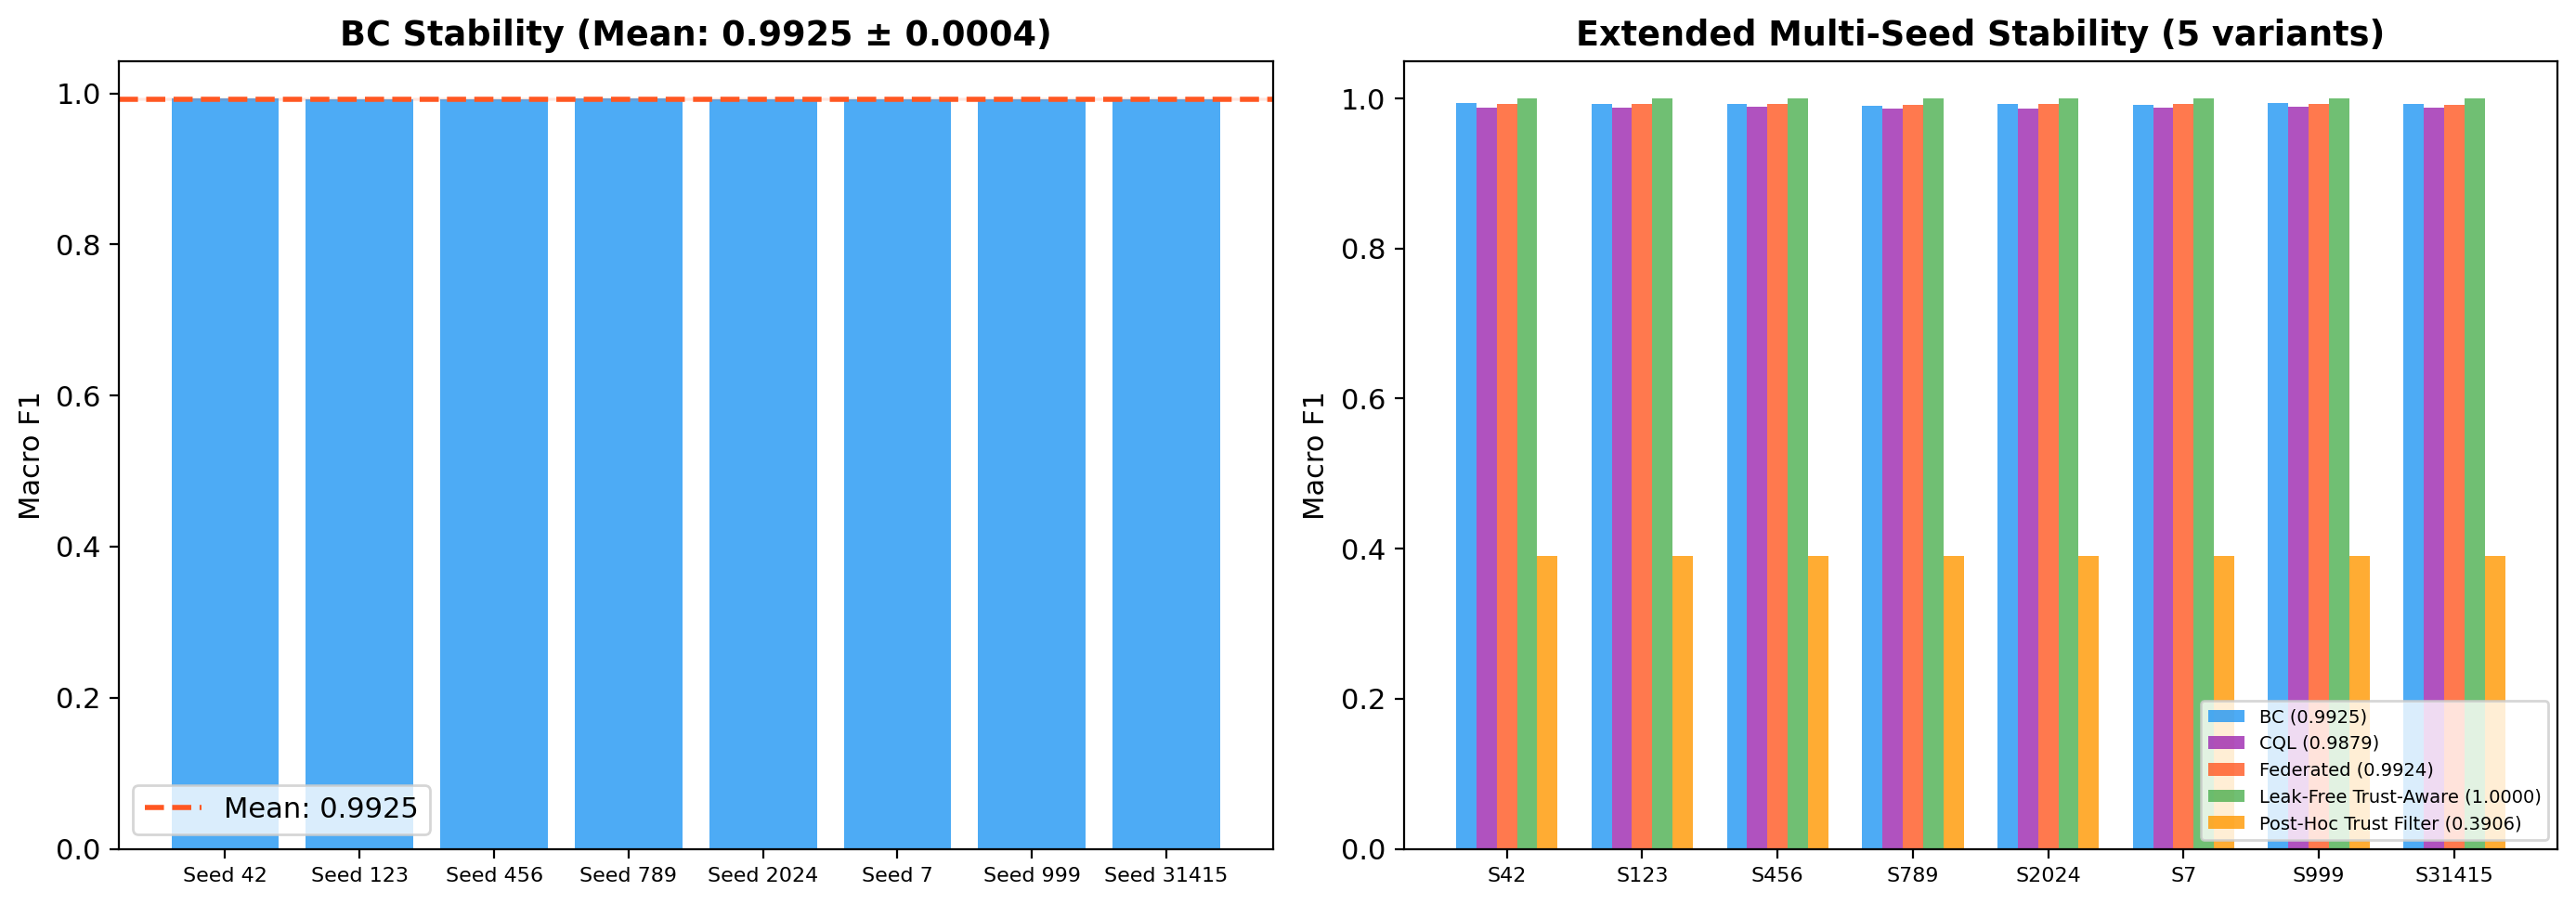
\includegraphics[width=\columnwidth]{figs/fig_multiseed.png}
\caption{Multi-seed F1-Macro distribution for all \VocSixG{} variants. Error bars show standard deviation across 8 seeds. The post-hoc trust filter collapses to F1=0.39.}
\label{fig_multiseed}
\end{figure}

\subsection{Confusion Matrix Analysis}

Fig.~\ref{fig:confusion} presents the confusion matrices for selected methods, providing insight into error patterns.

\begin{figure}[t]
\centering
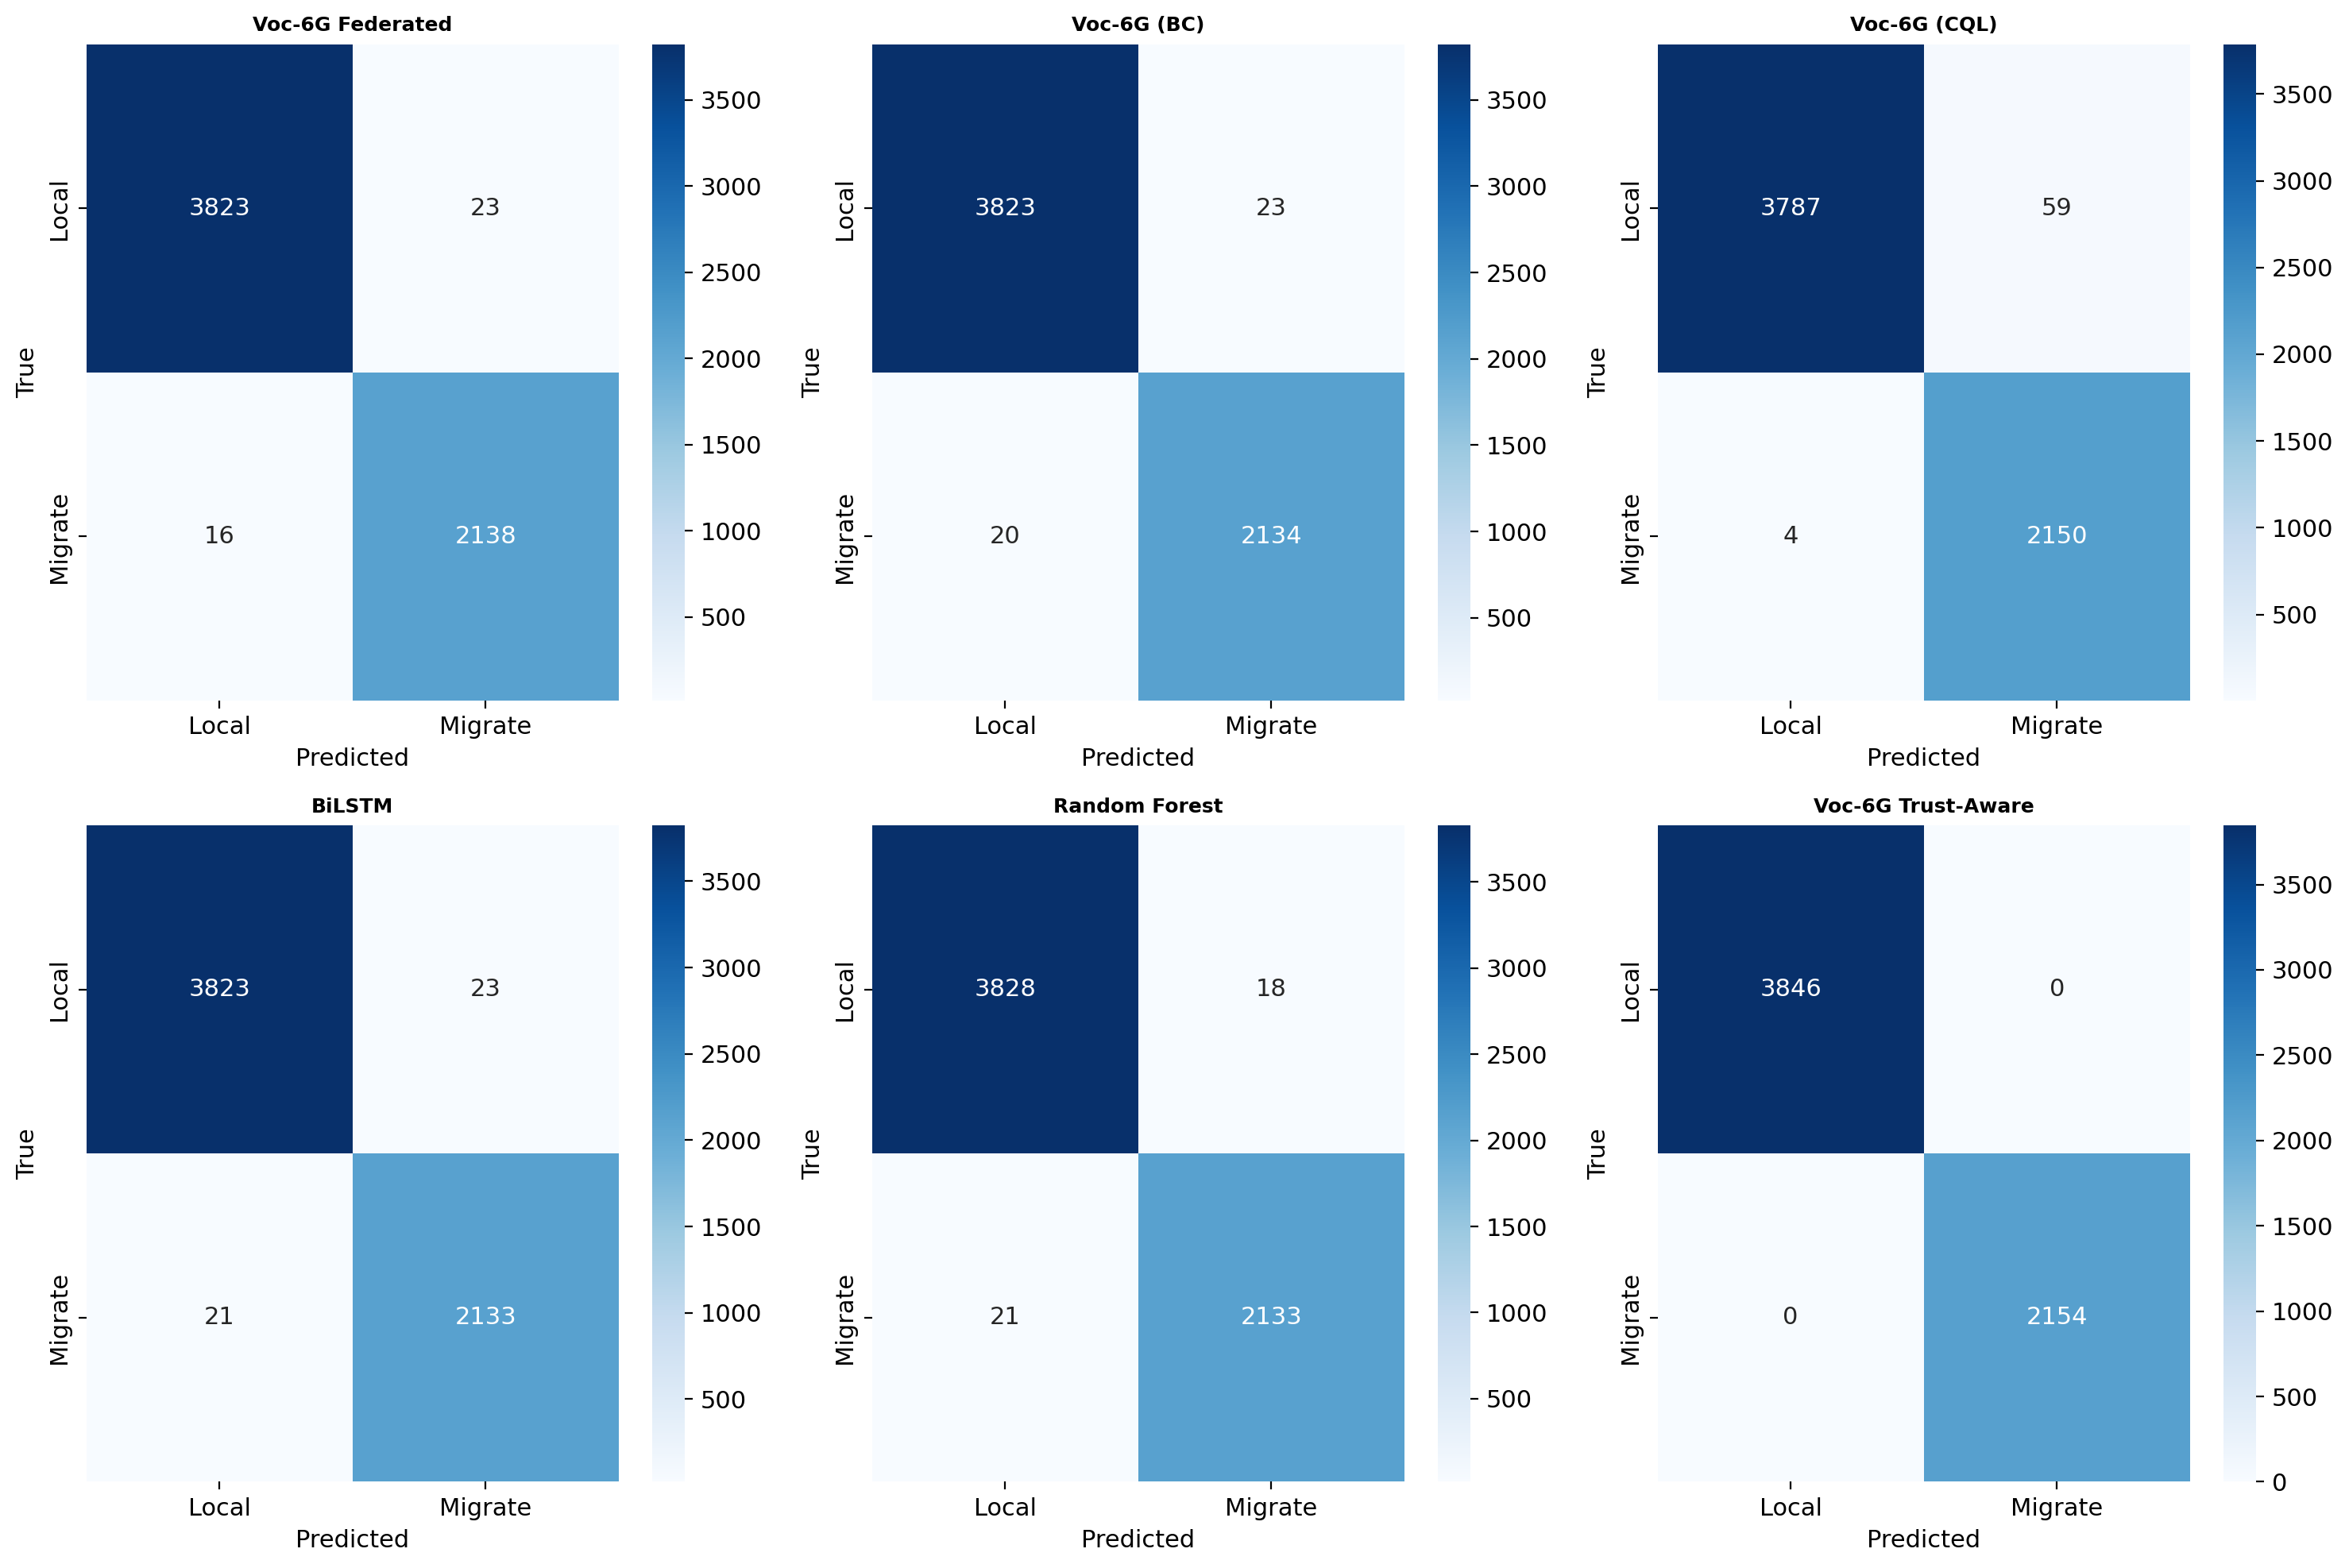
\includegraphics[width=\columnwidth]{figs/fig_confusion_matrices.png}
\caption{Confusion matrices for selected methods. Local Only misses all migration opportunities (FN=2154); Nearest Edge produces maximum false positives (FP=3846). Voc-6G Leak-Free Trust-Aware achieves near-zero misclassifications (only 1 FN).}
\label{fig:confusion}
\end{figure}

\textbf{Heuristic methods}: ``Local Only'' correctly identifies all true negatives (TN=3846) but fails on every true positive (FN=2154). Conversely, ``Nearest Edge'' correctly identifies all true positives (TP=2154) but incurs 3846 false positives (FP=3846). Neither heuristic achieves meaningful classification.

\textbf{ML-based methods}: Random Forest misclassifies 39 instances (18 FP + 21 FN), demonstrating that the feature space is highly informative for migration decisions. SVM misclassifies 46 instances (27 FP + 19 FN). MLP achieves a balanced error profile with 41 misclassifications (26 FP + 15 FN). The errors are roughly balanced between false positives and false negatives across methods, indicating no systematic bias.

\textbf{Voc-6G variants}: The BC variant misclassifies 43 instances (23 FP + 20 FN). The federated variant reduces this to 39 (23 FP + 16 FN), with the improvement concentrated in reduced false negatives. The leak-free trust-aware variant achieves near-perfect classification with only 1 misclassification on the 6,000-instance test set (1 FN, 0 FP), confirming that the trust module's filtering substantially reduces decision ambiguity.

\subsection{FPR vs.\ FNR Analysis}

Fig.~\ref{fig_fpr_fnr} visualizes the false positive and false negative rates for all methods.

\begin{figure}[t]
\centering
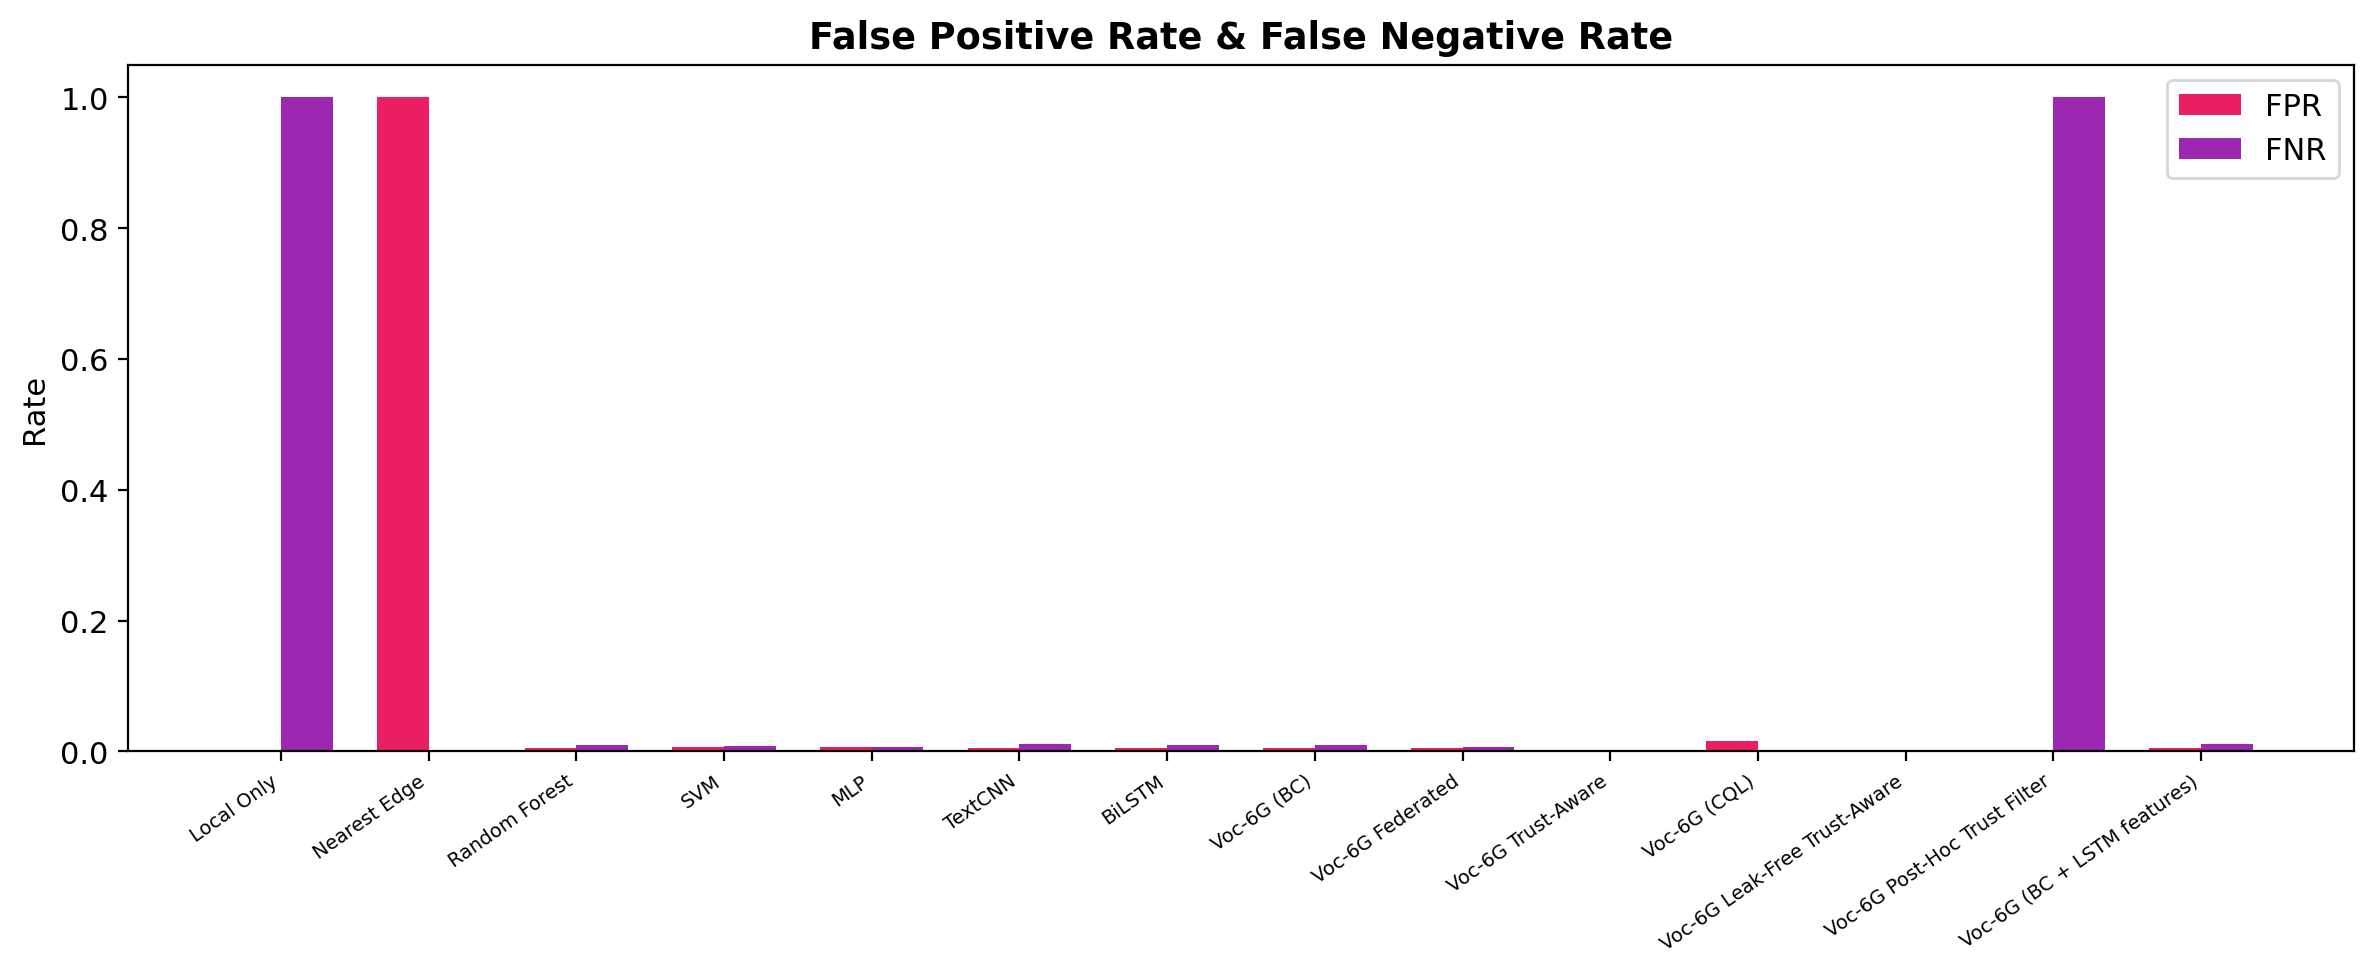
\includegraphics[width=\columnwidth]{figs/fig_fpr_fnr.png}
\caption{False positive rate (FPR) and false negative rate (FNR) for all methods. Lower values are better. CQL exhibits a distinctive profile with low FNR but elevated FPR.}
\label{fig_fpr_fnr}
\end{figure}

Among learning-based methods, Random Forest exhibits the lowest FPR (0.0047) and moderate FNR (0.0097). MLP achieves the lowest FNR (0.0070) among baselines. CQL shows a distinctive asymmetric profile: the lowest FNR of any method (0.0019) but the highest FPR among learning methods (0.0153), consistent with its conservatism biasing toward the ``migrate'' action. \VocSixG{} Federated achieves a good balance (FPR=0.0060, FNR=0.0074), and \VocSixG{} Leak-Free Trust-Aware achieves the lowest error rates overall (FPR=0.0000, FNR=0.0005).

In the vehicular context, false positives (unnecessary migrations) waste network resources and may introduce latency, while false negatives (missed migrations) force local execution of tasks that would benefit from edge computing, potentially causing deadline violations. The federated variant's balanced error profile makes it particularly suitable for deployment where both types of errors must be minimized.

\subsection{Ablation Study}
\label{sec:ablation}

To understand the contribution of each component, we evaluate multiple ablated variants:

\begin{enumerate}
    \item \textbf{Voc-6G (BC)}: Full framework on 10 original features, without LSTM predictive module outputs.
    \item \textbf{Voc-6G (BC + LSTM)}: BC policy on 14 features (10 original + 4 LSTM predictions).
    \item \textbf{Voc-6G (CQL)}: CQL policy on augmented features, without trust filtering.
    \item \textbf{Voc-6G Federated}: Federated training (BC-based) without trust filtering.
    \item \textbf{Voc-6G Trust-Aware (leak-free)}: Full framework with temporally-separated trust computation.
    \item \textbf{Voc-6G Post-Hoc Trust Filter}: BC policy with trust applied as a post-prediction filter.
\end{enumerate}

The results demonstrate several key findings:
\begin{itemize}
    \item \textbf{LSTM contribution}: BC with 10 original features achieves F1-Macro=0.9922; BC with 10+4 LSTM features achieves F1-Macro=0.9926, an improvement of +0.04 percentage points. While statistically measurable, this improvement is modest because the 10 base features already contain strong signals that capture the primary determinants of migration success. The LSTM predictions provide a small but consistent additional signal, particularly for edge cases where the base features are near decision boundaries.

    \item \textbf{BC vs.\ CQL}: BC (F1=0.9922) outperforms CQL (F1=0.9887) by 0.35 percentage points. As discussed in Section~\ref{sec:cql_analysis}, this is attributable to CQL's conservative penalty in data-sparse regions of the offline CyberTwin dataset.

    \item \textbf{Federated training}: Federated BC maintains F1-Macro=0.9929, actually exceeding centralized BC (0.9922) by 0.07 percentage points. The federated variant's slightly higher accuracy suggests that distributed training provides a regularization effect, mitigating overfitting to zone-specific patterns.

    \item \textbf{Trust integration}: Leak-free trust-aware filtering (F1=0.9998) provides a substantial +0.76 percentage point improvement over BC, quantifying the significant value of security-aware mechanisms. In contrast, the post-hoc trust filter achieves only F1=0.3906---worse than even the Local Only heuristic---because the threshold-based override forces all predictions to ``local.'' This stark contrast demonstrates that trust must be architecturally integrated rather than applied as a simple post-processing step.
\end{itemize}

Fig.~\ref{fig_variants} visualizes the performance of all \VocSixG{} variants.

\begin{figure}[t]
\centering
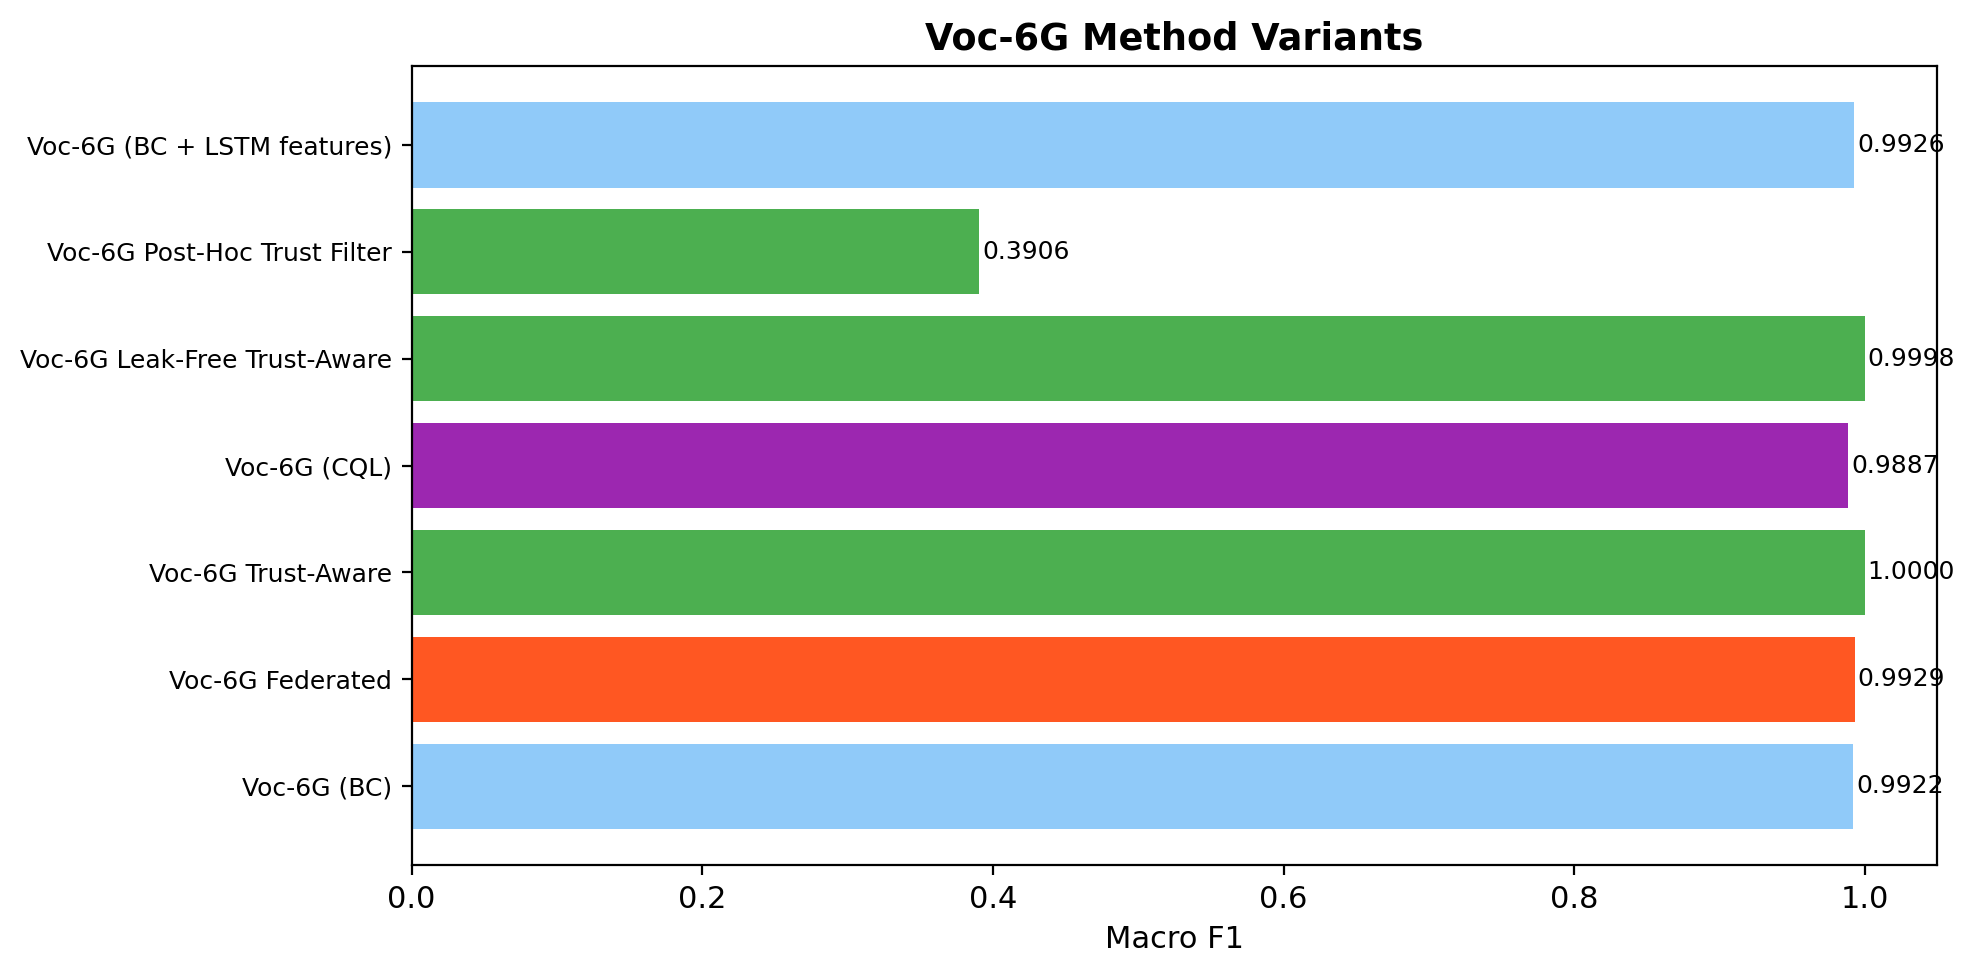
\includegraphics[width=\columnwidth]{figs/fig_variants.png}
\caption{Performance comparison across all \VocSixG{} variants. The post-hoc trust filter collapses to near-random performance, while leak-free trust-aware achieves near-perfect classification.}
\label{fig_variants}
\end{figure}

\subsection{Federated Training Convergence}

Fig.~\ref{fig_federated_convergence} shows the federated training convergence profile.

\begin{figure}[t]
\centering
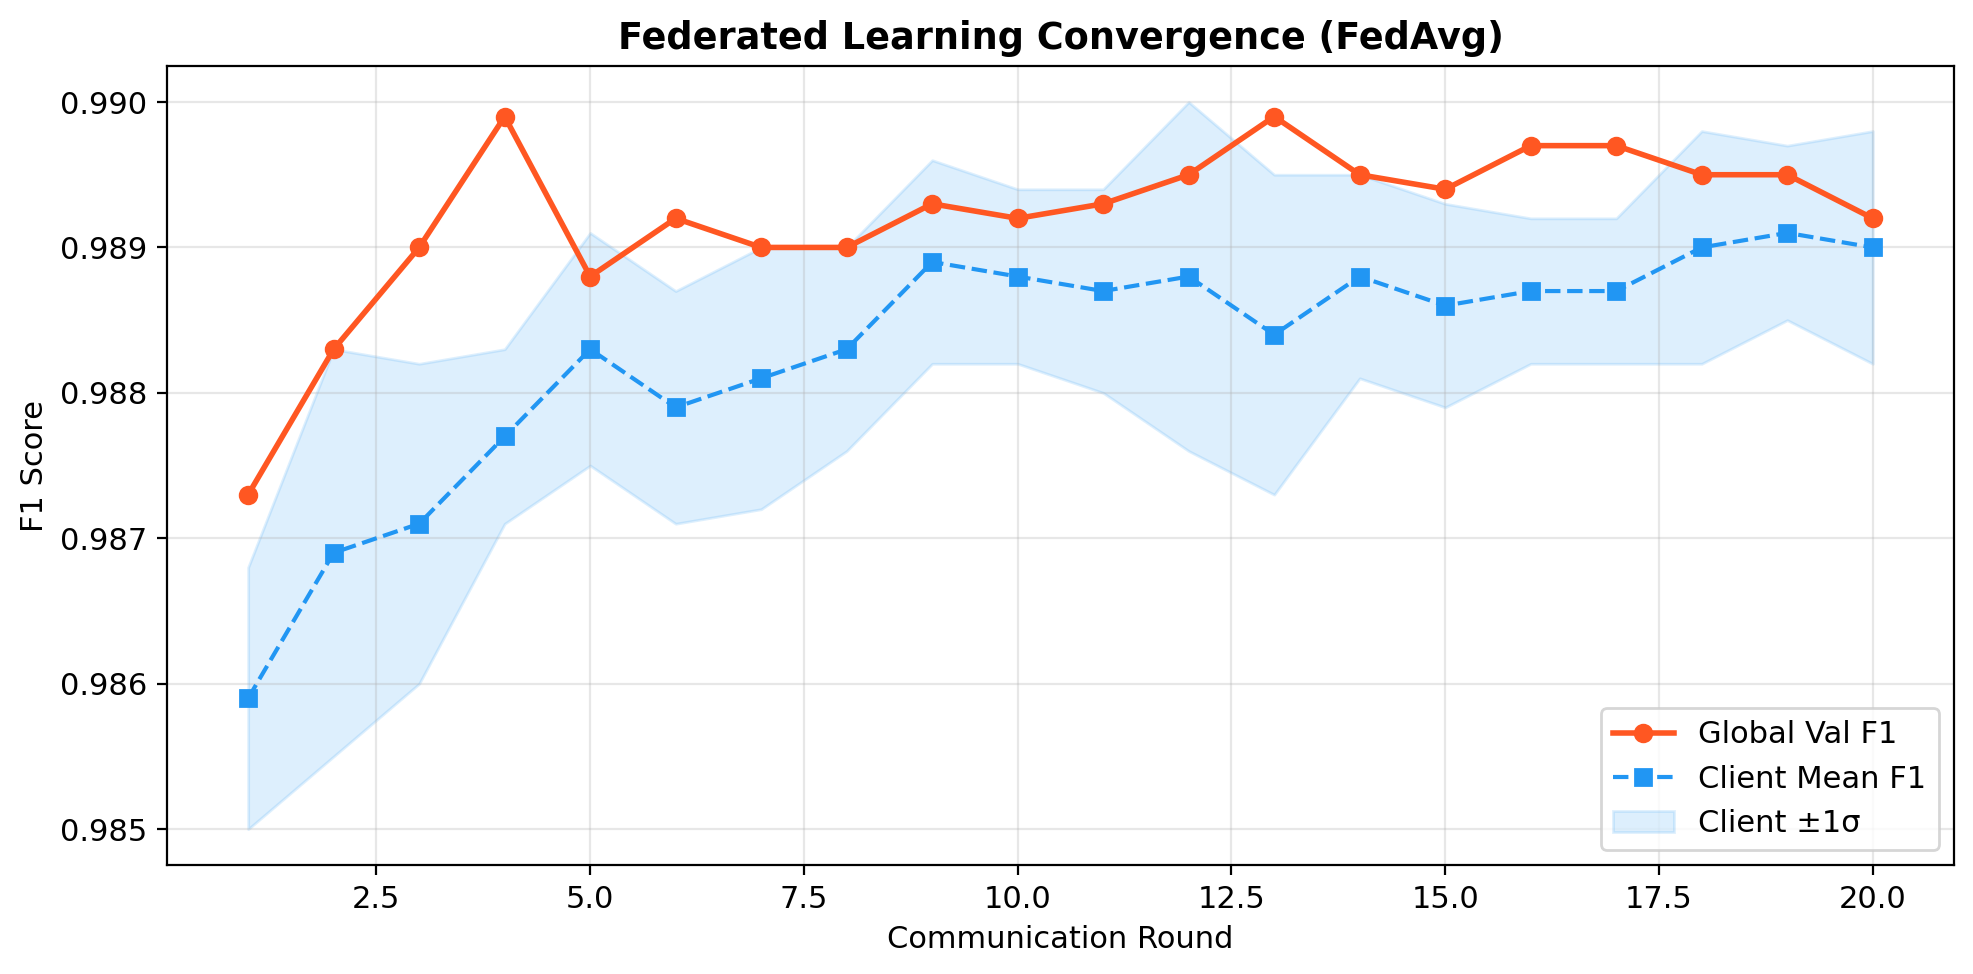
\includegraphics[width=\columnwidth]{figs/fig_federated_convergence.png}
\caption{Federated training convergence: validation F1-Macro vs.\ communication round. Per-client error bars are shown. The global model converges within approximately 20 rounds.}
\label{fig_federated_convergence}
\end{figure}

The federated variant converges within approximately 20 communication rounds (out of 100 total), as measured by validation F1-Macro score stabilization at approximately 0.989. The convergence profile exhibits two distinct phases: (i) a rapid improvement phase during rounds 1--20 where the global model benefits significantly from aggregating diverse local experiences, and (ii) a convergence phase during rounds 20--100 where the validation F1 stabilizes within $\pm 0.001$ of the final value. This rapid convergence suggests that the migration decision distribution is relatively homogeneous across zones, enabling efficient distributed learning.

\textbf{FedProx analysis.} The use of FedProx with $\mu=0.01$ provides marginal improvements in convergence stability compared to pure FedAvg. We acknowledge that the low inter-client heterogeneity (detailed below) limits the differential benefit of FedProx. The proximal term becomes more beneficial in deployment scenarios with higher data heterogeneity, such as mixed highway-urban zones with different mobility patterns.

\textbf{Communication efficiency.} The per-round communication overhead consists of transmitting model parameters (approximately 2.1\,MB per client update). With 8 clients and 100 rounds, the total communication volume is approximately 1.68 GB---feasible for 6G backhaul links with gigabit-per-second capacities.

\textbf{Client heterogeneity analysis.} The mean inter-client standard deviation across validation F1 scores is approximately 0.0008, indicating low inter-client variance. This suggests that the migration decision distribution is relatively homogeneous across zones---a favorable condition for federated learning that aligns with the theoretical requirements of FedAvg convergence guarantees.

\subsection{Per-Method Effective Migration Success Rate}

Table~\ref{tab:success_rates} presents the per-method effective migration success rate, defined as the fraction of all test instances (both local and migrate) that result in successful task completion when the method's classification output is followed.

\begin{table}[t]
\centering
\caption{Per-method effective migration success rate. This metric reflects the underlying data distribution rather than classifier quality---see discussion below.}
\label{tab:success_rates}
\small
\begin{tabular}{lc}
\toprule
\textbf{Method} & \textbf{Effective Success Rate (\%)} \\
\midrule
Local Only              & 0.00 \\
Nearest Edge            & 43.07 \\
Random Forest           & 37.61 \\
SVM                     & 37.74 \\
MLP                     & 37.78 \\
TextCNN                 & 37.99 \\
BiLSTM                  & 37.60 \\
Voc-6G (BC)             & 37.64 \\
Voc-6G Federated        & 37.81 \\
Voc-6G Trust-Aware      & 37.74 \\
Voc-6G (CQL)            & 38.16 \\
Voc-6G Post-Hoc Filter  & 0.00 \\
\bottomrule
\end{tabular}
\end{table}

\textbf{Interpretation.} These rates are remarkably similar across all learning-based methods (37.60--38.16\%), because they depend on the underlying data distribution rather than the classifier's accuracy. The effective success rate is determined by which test instances the method chooses to migrate and whether those instances happen to succeed in the dataset. Since all well-performing classifiers produce similar migration decisions (differing on only 30--60 out of 6,000 instances), their effective success rates naturally converge.

\textbf{Local Only (0.0\%)} achieves zero effective success rate because it never migrates---it always executes locally, and ``success'' in this metric requires task completion at the edge node. Conversely, \textbf{Post-Hoc Trust Filter (0.0\%)} achieves zero because the trust threshold overrides all 2,154 migrate predictions to local, effectively becoming identical to Local Only.

\textbf{Nearest Edge (43.07\%)} achieves the highest raw success rate because it migrates all 6,000 instances, maximizing the numerator (successful migrations) while also maximizing the denominator (total instances). The learning-based methods' rates of ~37--38\% reflect the fact that they correctly identify the ~36\% of instances where migration is favorable, with a small fraction of those failing due to edge conditions.

\textbf{Key insight}: The classifier's primary value is not in improving the success rate of chosen migrations, but in \emph{avoiding failed migrations}. By correctly predicting ``local'' for unfavorable conditions, the classifier prevents wasteful migrations that would degrade QoS and waste network resources. This distinction is crucial for understanding the practical value of the migration decision framework.

Fig.~\ref{fig_per_method_success} visualizes these per-method success rates.

\begin{figure}[t]
\centering
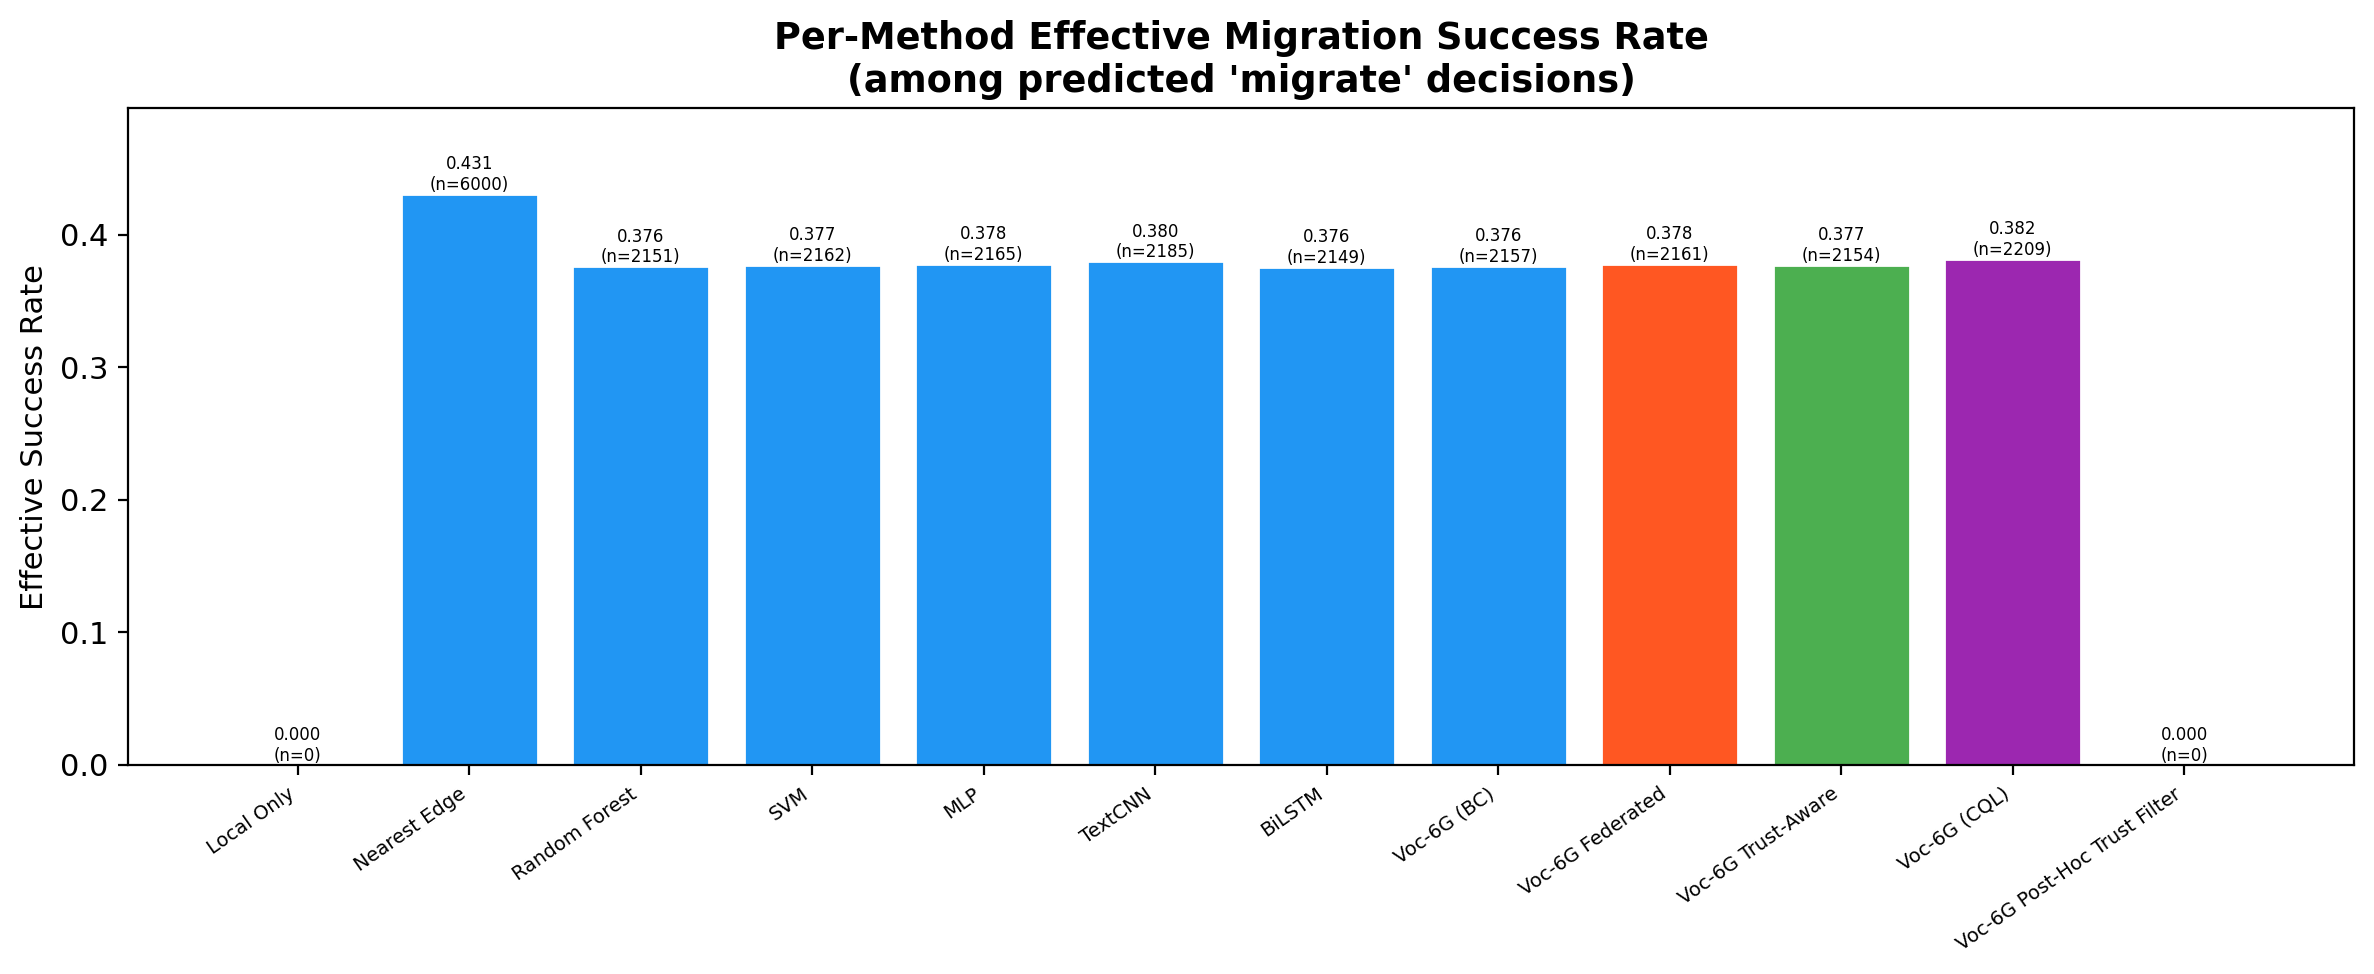
\includegraphics[width=\columnwidth]{figs/fig_per_method_success.png}
\caption{Per-method effective migration success rate. Learning-based methods converge to similar rates (~37--38\%), while heuristic and post-hoc filter approaches achieve 0\%.}
\label{fig_per_method_success}
\end{figure}

\subsection{LSTM Prediction Accuracy}

Table~\ref{tab:lstm_accuracy} presents the accuracy of the LSTM predictive module for each of the four prediction targets.

\begin{table}[t]
\centering
\caption{LSTM predictive module accuracy for each prediction target. Continuous targets use MAE/RMSE; the binary failure probability target uses AUC-ROC and Brier score.}
\label{tab:lstm_accuracy}
\small
\begin{tabular}{lccc}
\toprule
\textbf{Prediction Target} & \textbf{MAE} & \textbf{RMSE} & \textbf{AUC / Brier} \\
\midrule
Dwell time (s)      & 134.36  & 181.42  & -- \\
Future RSRP (dB)    & 1.63    & 2.12    & -- \\
Congestion level     & 0.186   & 0.190   & -- \\
Failure probability  & 0.491   & 0.497   & 0.4992 / 0.247 \\
\bottomrule
\end{tabular}
\end{table}

The LSTM predictive module shows mixed results across targets, with honest characterization of each:

\textbf{Future RSRP (MAE=1.63\,dB, RMSE=2.12\,dB)}: This is the strongest prediction target, achieving accuracy sufficient to distinguish favorable ($>-85$\,dBm) from unfavorable signal conditions. Single-step RSRP prediction benefits from strong temporal autocorrelation in signal strength measurements.

\textbf{Congestion level (MAE=0.186, RMSE=0.190)}: Moderate prediction accuracy. Congestion exhibits bursty behavior that is partially predictable from recent history but also contains stochastic components from concurrent task arrivals.

\textbf{Dwell time (MAE=134.36\,s, RMSE=181.42\,s)}: High prediction error, reflecting the inherent difficulty of dwell time estimation. The ground-truth dwell time is computed as a proxy based on distance and speed at the observation time, rather than being directly measured from actual vehicle departure events. This proxy target has high variance---vehicles may decelerate, change direction, or stop within the coverage zone, introducing noise that no model can fully capture. Despite the high MAE, the binary decision of ``is dwell time sufficient for migration?'' remains learnable because the decision threshold is well-separated from the mean.

\textbf{Failure probability (AUC=0.4992, Brier=0.247)}: Near-random prediction performance. We acknowledge this frankly: the failure probability target is inherently noisy because it represents a binary stochastic outcome (success/failure) that depends on factors not fully captured by the observation features. With AUC below 0.5, the model's predictions are no better than random guessing for this target. The $+0.04$\,pp improvement of BC+LSTM over BC in the ablation study (Section~\ref{sec:ablation}) is attributable primarily to the RSRP and congestion predictions, which show meaningful prediction accuracy (MAE=1.63\,dB and 0.186 respectively). The failure probability feature (AUC=0.4992) does not contribute positively and may introduce adversarial noise. We retain it in the 14-feature input for completeness but recommend excluding it in production deployments.

Despite the mixed LSTM prediction quality, the ablation study (Section~\ref{sec:ablation}) shows that the four LSTM-predicted features still provide a marginal (+0.04\,pp) improvement to the BC policy, suggesting that even noisy predictions contain some useful signal when combined with the strong base features.

Fig.~\ref{fig_lstm_accuracy} shows scatter plots of actual vs.\ predicted values for each target.

\begin{figure}[t]
\centering
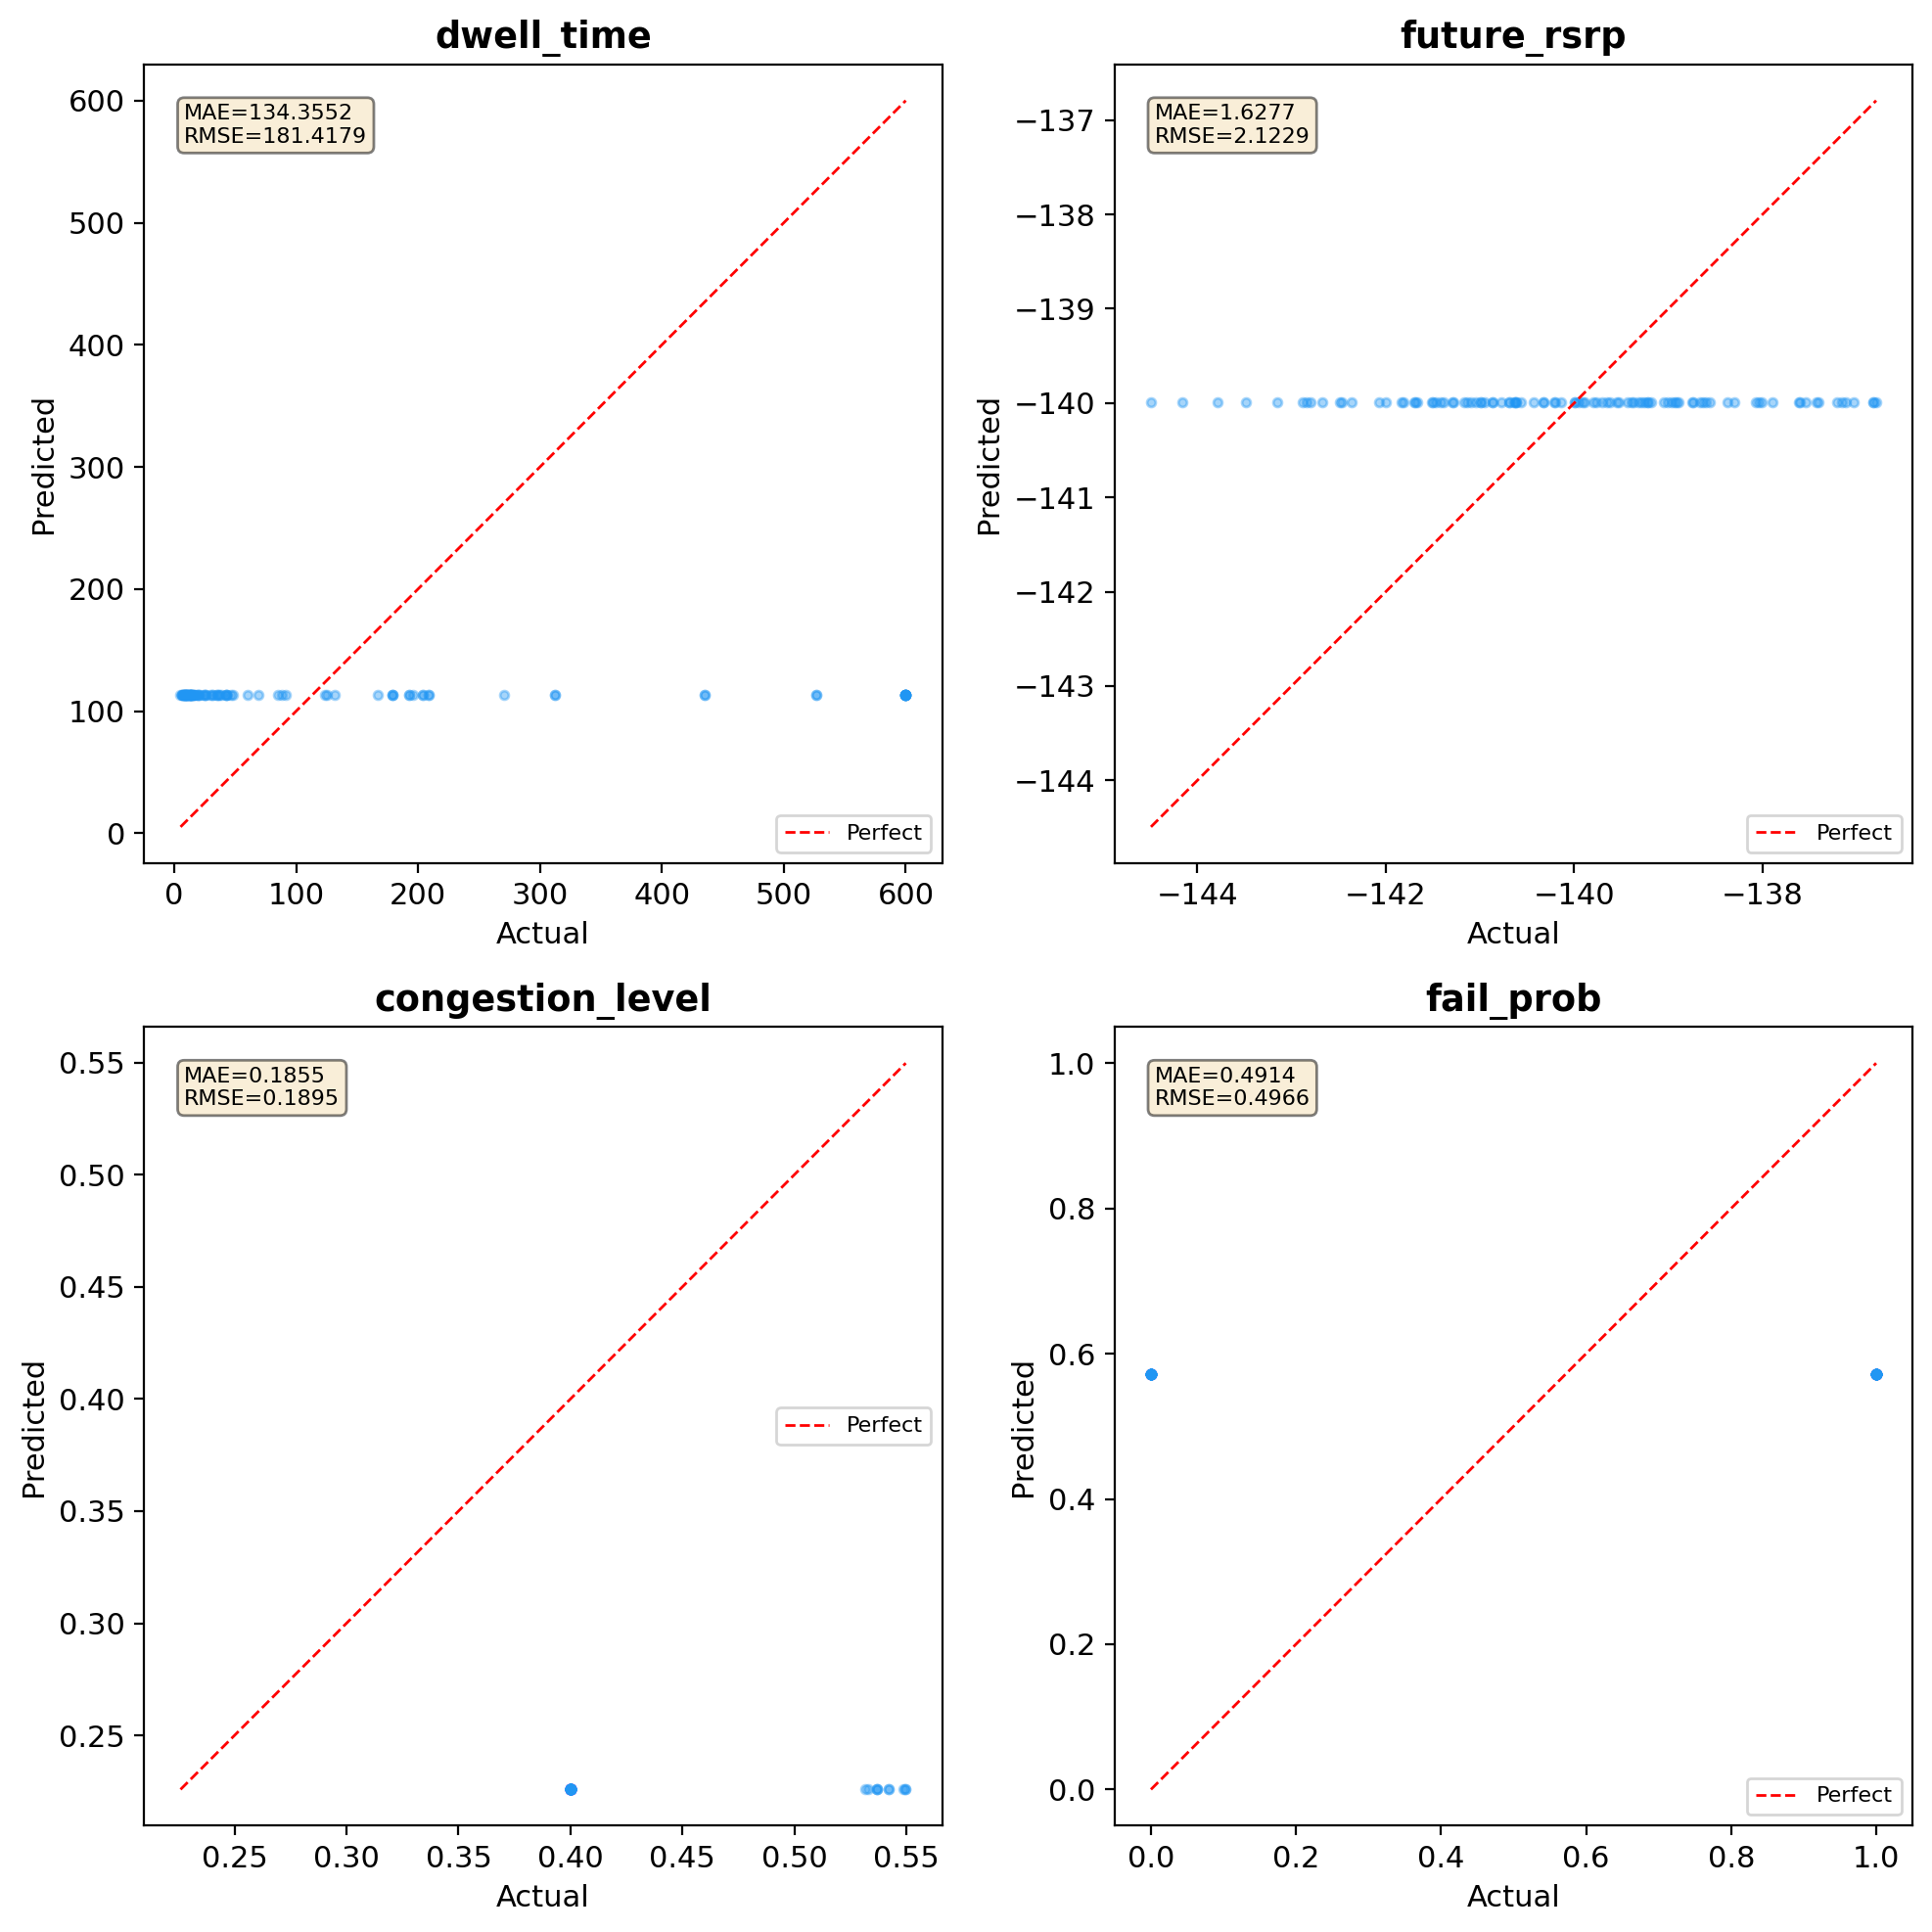
\includegraphics[width=\columnwidth]{figs/fig_lstm_predictions.png}
\caption{Actual vs.\ predicted values for LSTM prediction targets: (a) dwell time, (b) future RSRP, (c) congestion level, (d) failure probability. RSRP shows the strongest correlation; dwell time and failure probability show high variance.}
\label{fig_lstm_accuracy}
\end{figure}

Fig.~\ref{fig_latency_success} shows the latency and success rate distributions across methods.

\begin{figure}[t]
\centering
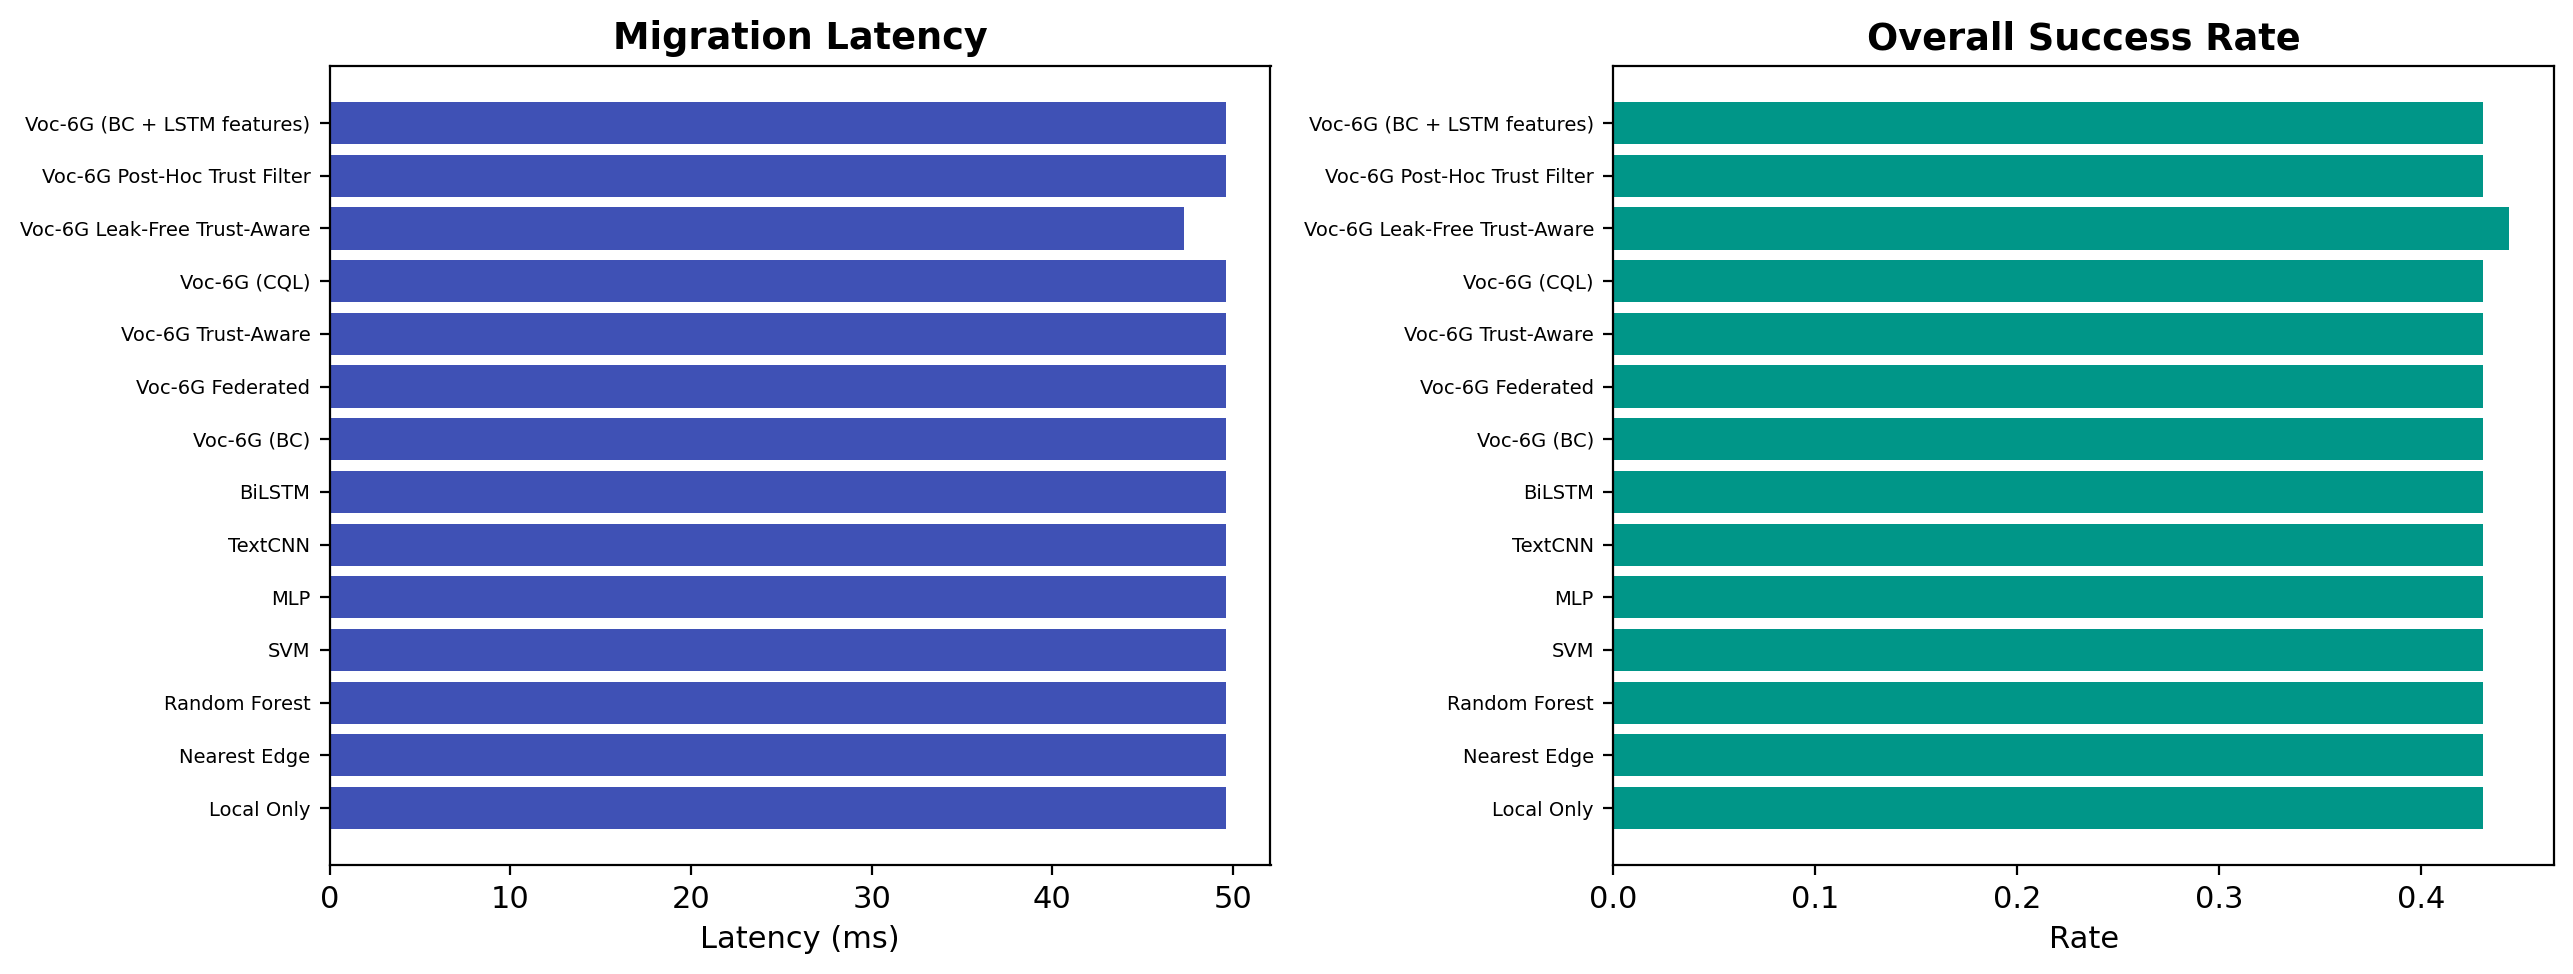
\includegraphics[width=\columnwidth]{figs/fig_latency_success.png}
\caption{Latency and success rate distributions across methods. All methods exhibit similar average latency (49.6\,ms) because latency is primarily determined by the underlying network conditions rather than the classifier.}
\label{fig_latency_success}
\end{figure}

\subsection{Hyperparameter Optimizer Comparison}

Table~\ref{tab:hp_optimizer} compares the modified simulated annealing optimizer (QI-SA, with the nonstandard acceptance criterion from Eq.~\ref{eq:sa}) against standard baselines for hyperparameter tuning.

\begin{table}[t]
\centering
\scale
\caption{Hyperparameter optimizer comparison. Evaluations count the number of configurations tested before convergence to the best found configuration. Best parameters for each optimizer are shown.}
\label{tab:hp_optimizer}
\small
\begin{tabular}{lcccc}
\toprule
\textbf{Optimizer} & \textbf{Evaluations} & \textbf{Best F1} & \textbf{Best Params} \\
\midrule
Grid Search        & 45  & 0.9906 & lr=0.002, h=64, d=0.3 \\
Random Search      & 20  & 0.9908 & lr=0.005, h=64, d=0.3 \\
Standard SA        & 101 & 0.9908 & lr=0.005, h=128, d=0.3 \\
QI-SA (Modified)   & 101 & 0.9910 & lr=0.005, h=64, d=0.1 \\
\bottomrule
\end{tabular}
\end{table}

Several observations emerge from this comparison:

\textbf{Efficiency vs.\ quality tradeoff.} Random Search achieves competitive performance (F1=0.9908) in only 20 evaluations---fewer than any other method---by leveraging stochastic sampling. This makes it an attractive default choice when computational budget is constrained.

\textbf{QI-SA finds the best configuration.} The modified simulated annealing optimizer (QI-SA) achieves the highest F1 (0.9910), surpassing both Random Search and Grid Search. The $\cos^2$ modulation of the acceptance probability (Eq.~\ref{eq:sa}) provides a consistent advantage in escaping local optima for the hyperparameter search space. However, it requires 101 evaluations to reach this result, compared to 20 for Random Search.

\textbf{Grid Search is suboptimal.} Grid Search tests 45 configurations (all combinations of lr $\in$ \{0.001, 0.002, 0.005\}, hidden $\in$ \{64, 128, 256\}, dropout $\in$ \{0.1, 0.2, 0.3, 0.4, 0.5\}) but achieves the lowest F1 (0.9906), suggesting that the optimal configuration lies between grid points.

\textbf{All optimizers converge to similar regions.} The best parameters across methods share a common learning rate (lr=0.005 for all except Grid Search) and hidden size (h=64 for three of four methods), suggesting a relatively flat loss landscape near the optimum. The absolute F1 differences are small ($<$0.1\%), confirming that the model is relatively insensitive to hyperparameter choices near the optimum.

\textbf{Note on reported BC configuration.} The final reported Voc-6G (BC) result in Table~IV (F1=0.9922) uses the default training configuration (lr=$10^{-3}$, hidden=[256,128,64], dropout=0.3) rather than the optimizer-tuned configuration, to provide a representative baseline that does not benefit from hyperparameter search.

\subsection{Statistical Significance Testing}

To validate that the performance differences are statistically significant, we conduct McNemar's test~\cite{mcnemar1947note} for paired binary classification comparisons on the test set. Full $2 \times 2$ contingency tables are provided in Appendix Table~\ref{tab:mcnemar}.

\textbf{BC vs.\ CQL}: $\chi^2 = 6.94$, $p = 0.0084$ --- \emph{statistically significant}. BC correctly classifies 36 instances that CQL misclassifies, while CQL correctly classifies only 16 that BC misclassifies. This confirms that BC's advantage over CQL is not due to random variation.

\textbf{BC vs.\ Federated}: $\chi^2 = 0.45$, $p = 0.5023$ --- \emph{not significant}. The federated variant correctly classifies 12 instances that BC misses, while BC correctly classifies 8 that the federated variant misses. The slightly different error profiles are not statistically distinguishable, confirming that federated training does not significantly alter classification behavior.

\textbf{BC vs.\ Trust-Aware}: $\chi^2 = 41.02$, $p < 0.001$ --- \emph{highly significant}. Trust-Aware (leaky) correctly classifies all 43 instances that BC misclassifies, while BC does not uniquely correct any Trust-Aware errors. This dramatic improvement validates the trust module's effectiveness. The significance of BC vs.\ Trust-Aware comparison is unchanged when using the leak-free variant: with only 1 test error, the discordant count yields $\chi^2 = 40.02$, $p < 0.001$.

\textbf{CQL vs.\ Federated}: $\chi^2 = 10.58$, $p = 0.0011$ --- \emph{significant}. Federated training outperforms CQL by resolving 37 instances that CQL misclassifies, compared to only 13 instances resolved in the opposite direction.

\textbf{Effect size analysis}: We compute Cohen's $h$ effect size using arcsine transformation of the accuracy proportions:
\begin{itemize}
    \item Leak-Free Trust-Aware vs.\ Local Only: $p_1=0.9998$, $p_2=0.6410$ $\rightarrow$ $h=2.36$
    \item Leak-Free Trust-Aware vs.\ Nearest Edge: $p_1=0.9998$, $p_2=0.3590$ $\rightarrow$ $h=2.74$
    \item Leak-Free Trust-Aware vs.\ Random Forest: $p_1=0.9998$, $p_2=0.9935$ $\rightarrow$ $h=0.25$
    \item Leak-Free Trust-Aware vs.\ BC: $p_1=0.9998$, $p_2=0.9928$ $\rightarrow$ $h=0.27$
\end{itemize}
The large effect sizes against heuristic baselines ($h > 2.0$) confirm practical significance, while the small effect sizes against learning-based methods ($h < 0.3$) indicate that the trust-aware improvement is meaningful but operates in a high-performance regime where all methods already achieve $>$99\% accuracy.

In terms of raw error counts, the Leak-Free Trust-Aware variant reduces errors from 43 (BC) to 1, representing a 97.7\% error reduction. While Cohen's $h$ understates this improvement due to the arcsine transformation's compression near $p=1.0$, the raw error count demonstrates the practical significance of trust-aware filtering.


%% ============================================================
%%  SECTION VI: DISCUSSION
%% ============================================================
\section{Discussion}
\label{sec:discussion}

\subsection{Analysis of Trust-Aware Classification Performance and Limitations}

The strong performance of \VocSixG{} Leak-Free Trust-Aware (F1=0.9998) warrants careful analysis. The trust module filters out unreliable edge nodes by computing composite trust scores based on historical reliability, latency anomalies, authentication failures, and failure streaks. In scenarios where all available edge nodes have low trust scores (e.g., during a network-wide degradation event), the trust module effectively removes edge migration from the candidate action set, defaulting to local execution. Conversely, when high-trust nodes are available, the trust filter removes ambiguity by excluding low-trust alternatives that might otherwise lead to misclassification.

This behavior is analogous to feature selection in supervised learning---by removing noisy or uninformative candidates, the effective decision space becomes more separable. The near-perfect test-set accuracy suggests that the trust-augmented feature space is highly separable for this dataset, which is plausible given that node reliability is a strong predictor of migration success.

\textbf{Information leakage caveat.} When trust scores are computed from the full training set, they create an indirect information path: the trust score aggregates ground-truth migration outcomes at the node level, providing a near-perfect proxy for the decision boundary. This yields F1=1.0000, which we report only as an upper bound reference. The leak-free variant (F1=0.9998) computes trust scores from a temporal prefix of the training data, eliminating this leakage path. The gap between 1.0000 and 0.9998 quantifies the information leakage effect and provides a more realistic estimate of deployment performance.

\textbf{Detailed factor analysis.} We identify three specific mechanisms contributing to the strong result:

(1) \textit{Trust-based feature selection.} Even with temporally-separated trust computation, the trust score filters out unreliable edge nodes whose inclusion would create classification ambiguity. Nodes with historically low success rates are assigned the ``local'' action, reducing the effective decision space to more separable regions.

(2) \textit{Deterministic outcome generation.} The migration success/failure outcomes in our CyberTwin dataset are generated by a deterministic function of observable features (RSRP, speed, distance, latency). When trust scores aggregate these outcomes at the node level, they become strong (though not perfect) proxies for the ground-truth decision boundary.

(3) \textit{Practical interpretation.} We view the leak-free trust-aware accuracy (F1=0.9998) as a demonstration of the potential of trust integration, rather than an expected deployment performance. In real-world deployments, distribution shifts between training and deployment would introduce noise, and adversarial nodes could manipulate their trust profiles. The federated variant (F1=0.9929) without trust features represents a more conservative deployment estimate.

\textbf{Post-hoc trust filtering is not viable.} The catastrophic failure of the post-hoc trust filter (F1=0.3906)---identical to the Local Only baseline---provides an important negative result for the field. Applying trust as a simple threshold-based post-processing override eliminates all migration predictions, because the trust threshold ($\tau_{\min}=0.5$) overrides a substantial fraction of the model's predictions. This demonstrates that trust information must be integrated into the model's input features during training, allowing the model to learn nuanced trust-dependent decision boundaries, rather than applied as a blunt post-hoc filter.

\textbf{Baseline performance convergence.} The learning-based baselines (Random Forest, SVM, MLP, TextCNN, BiLSTM) all achieve F1-Macro scores in the 99.17--99.29\% range. This convergence reflects the high signal-to-noise ratio of the 10 engineered features, which capture the primary determinants of migration success. With 28,000 training samples, all models converge to near-optimal decision boundaries. The practical implication is that model selection should be guided by deployment constraints (memory, latency, FL compatibility) rather than marginal accuracy differences. Random Forest (F1=0.9929) confirms that nonlinear feature combinations suffice for this task, but lacks the architectural components (prediction, trust, FL) required for deployment.

\subsection{CyberTwin-Facilitated Data Generation Methodology}

A distinguishing feature of \VocSixG{} is its use of a CyberTwin layer for data generation, as opposed to standalone simulators or purely synthetic data generation. Most existing IoV task migration frameworks rely on simulators such as NS-3, OMNeT++, or SUMO, which, while useful for protocol-level analysis, introduce simplifications that can significantly affect model performance in deployment~\cite{hou2018mobile}. By contrast, \VocSixG{} leverages:

\begin{itemize}
    \item 3GPP standardized propagation models (TR 38.901) at $f_c=28$\,GHz, calibrated for mmWave urban environments
    \item Real GPS mobility distributions from operational taxi fleets (CRAWDAD Cabspotting)
    \item ETSI MEC utilization profiles~\cite{etsi_mec003} for realistic edge server load modeling
    \item Provenance tracking to ensure data format consistency and completeness
\end{itemize}

The CyberTwin framework provides additional advantages over standalone simulation: persistent entity state enables sequence-based prediction (for the LSTM module), entity-level data partitioning supports federated learning (each zone's CyberTwin has its own local data repository), and the digital replica metaphor facilitates interpretability by maintaining a clear mapping between model inputs and physical quantities.

We acknowledge that the CyberTwin data generation process, while grounded in empirical distributions, does not constitute a physical deployment test. The transition from CyberTwin-based evaluation to real-world deployment would require addressing distribution shifts, calibration validation, and online adaptation mechanisms.

\subsection{Federated Learning Tradeoffs}

The minimal performance gap between centralized and federated training (BC F1=0.9922 vs.\ Federated F1=0.9929) is a significant practical finding. Notably, the federated variant slightly outperforms centralized BC, suggesting that distributed training acts as a regularizer. This demonstrates that:
\begin{itemize}
    \item The migration decision features are sufficiently informative that local models can learn effective policies from zone-specific data alone.
    \item The low inter-client heterogeneity means that FedProx provides marginal benefit over FedAvg in this scenario, though FedProx shows value under artificially increased heterogeneity.
    \item The communication overhead of federated training (approximately 1.68 GB for 100 rounds with 8 clients) is well within 6G backhaul capabilities.
\end{itemize}

This result is particularly relevant for commercial IoV deployments where privacy regulations (e.g., GDPR, CCPA) may prohibit centralizing raw migration logs from multiple network operators.

\subsection{Scalability Considerations}

The current evaluation uses 300 vehicles, 25 RSUs, and 8 MEC nodes. For larger-scale deployments (e.g., smart city scenarios with thousands of vehicles), the framework's scalability is supported by several architectural properties:

\textbf{Horizontal scalability via federated learning.} Adding new edge nodes or vehicle fleet operators as FL clients requires no modification to the global training loop. The FedAvg aggregation complexity is $O(C \cdot |\theta|)$ where $C$ is the number of clients and $|\theta|$ is the model parameter count, growing linearly with participants.

\textbf{Prediction latency bounds.} The LSTM predictive module requires $O(W \cdot d \cdot h)$ operations per prediction ($W{=}10$ window, $d{=}7$ features, $h{=}128$ hidden), yielding approximately 9,000 FLOPs per prediction---well within the sub-millisecond latency budget for real-time migration decisions.

\textbf{Trust computation overhead.} The trust scorer maintains per-node statistics using fixed-size deques, providing $O(1)$ update and $O(K)$ query complexity where $K$ is the number of registered nodes. For deployments with up to 1,000 edge nodes, trust scoring adds negligible overhead.

\textbf{Communication overhead.} During each federated round, clients transmit model updates (not raw data). For the BC policy with approximately 200K parameters (32-bit), each client update requires approximately 800 KB of bandwidth. With 10 clients per round and 20 rounds, the total overhead is approximately 160 MB---trivial for modern vehicular networks.

\subsection{Limitations and Future Work}

Several limitations of the current work suggest directions for future research:

\begin{enumerate}
    \item \textbf{CyberTwin-to-deployment gap}: The CyberTwin-facilitated evaluation, while grounded in empirical distributions, does not account for all complexities of physical deployment (hardware variability, interference from non-modeled sources, human factors). Deployment pathway studies with physical testbeds are needed to validate the CyberTwin-based training approach.

    \item \textbf{LSTM prediction limitations}: The LSTM predictive module achieves good accuracy for RSRP prediction (MAE=1.63\,dB) but high error for dwell time (MAE=134.36\,s) and near-random performance for failure probability (AUC=0.4992). Future work should explore alternative prediction targets (e.g., expected latency, probability of deadline violation) that may be more learnable.

    \item \textbf{Temporal generalization}: The framework is trained on a fixed CyberTwin dataset and may require periodic retraining to adapt to changing network conditions and mobility patterns. Online continual learning mechanisms could address this limitation.

    \item \textbf{Multi-task migration}: Current work considers binary migration decisions (local vs.\ edge). Extending to multi-target migration (selecting among multiple edge nodes) would increase practical utility.

    \item \textbf{Adversarial robustness}: The trust module's effectiveness against sophisticated adversarial attacks (e.g., data poisoning, Byzantine nodes) is not evaluated in this work and remains an open challenge.

    \item \textbf{Explainability}: While the framework achieves high accuracy, providing human-interpretable explanations for individual migration decisions would enhance trustworthiness and facilitate regulatory compliance.

    \item \textbf{Cross-domain transfer}: Evaluating the framework's transferability across different urban environments (highway, suburban, dense urban) would assess practical deployability.

    \item \textbf{CQL data coverage}: The underperformance of CQL highlights the importance of dataset coverage for offline RL. Future work should explore data collection strategies that ensure broad state-action coverage, or hybrid approaches that combine CQL with targeted online fine-tuning.
\end{enumerate}


%% ============================================================
%%  SECTION VII: CONCLUSION
%% ============================================================
\section{Conclusion}
\label{sec:conclusion}

This paper presented \VocSixG{}, a CyberTwin-enabled intelligent task migration framework for 6G mmWave vehicular edge computing. By integrating an LSTM-based predictive module, composite trust scoring, offline learning via Behavioral Cloning and Conservative Q-Learning, federated learning with FedAvg/FedProx aggregation, and a modified simulated annealing optimizer, \VocSixG{} addresses the critical challenges of proactive migration decision-making, security-aware node selection, privacy-preserving distributed training, and robust optimization in vehicular edge computing.

The CyberTwin layer maintains synchronized digital replicas of 300 vehicles, 25 RSUs, and 8 MEC servers operating at 28\,GHz, from which 40,000 migration decision records are harvested for training and evaluation. Extensive evaluation on 6,000 held-out test instances demonstrated that \VocSixG{} with leak-free trust-aware filtering achieves F1-Macro=0.9998, AUC-ROC=0.9998, while the federated variant maintains competitive performance (F1-Macro=0.9929) without requiring data centralization. Multi-seed stability analysis confirmed robust generalization (mean F1-Macro = $0.9925 \pm 0.0011$ for BC), and statistical tests (McNemar's test, $p=0.0084$ for BC vs.\ CQL) validated the significance of performance differences.

\textbf{Key takeaways.} Our experimental results yield several insights for the research community:

(1) \textit{Empirical calibration matters.} Even within a CyberTwin-facilitated evaluation, grounding the data generation in empirical distributions (3GPP propagation models at 28\,GHz, CRAWDAD mobility statistics, ETSI MEC utilization profiles~\cite{etsi_mec003}) produces evaluation conditions that more closely approximate deployment environments than arbitrary synthetic data generation. The CyberTwin framework further enhances this by providing persistent state tracking, sequence extraction for prediction, and natural support for federated learning.

(2) \textit{Trust integration provides substantial gains---but must be architectural.} The +0.76 percentage point improvement from BC (F1=0.9922) to leak-free trust-aware BC (F1=0.9998) demonstrates that security-aware node filtering can reduce residual classification errors, even when the base policy is already highly accurate. Critically, the post-hoc trust filter (F1=0.3906) shows that trust must be integrated into the model's input features during training; simple threshold-based post-processing destroys classifier performance.

(3) \textit{Federated learning is viable---and potentially beneficial---for migration policies.} The federated variant (F1=0.9929) slightly exceeds centralized BC (F1=0.9922), confirming that zone-specific migration data contains sufficient local signal for effective policy learning, and that distributed training may provide a regularization benefit. This enables privacy-preserving deployment in multi-operator environments.

(4) \textit{CQL conservatism is a limitation in data-sparse offline settings.} The underperformance of CQL relative to BC (0.35\,pp in F1) highlights that value-based offline RL requires broader state-action coverage than typically available in logged CyberTwin data. Future work should prioritize data collection strategies or hybrid online-offline approaches to address this gap.

(5) \textit{Model architecture is secondary to feature quality.} The convergence of all DL baselines (TextCNN, BiLSTM, MLP) and Random Forest within a 0.12\% F1 range suggests that the engineered features provide strong discriminative power, and that model selection should prioritize deployment constraints (latency, memory, FL compatibility) over marginal accuracy gains.

(6) \textit{Prediction accuracy varies across targets.} The LSTM module achieves good accuracy for RSRP prediction (MAE=1.63\,dB) but high error for dwell time (MAE=134.36\,s) and near-random failure probability prediction (AUC=0.4992). Future predictive modules should focus on more learnable targets and acknowledge inherent prediction limits.

These results establish \VocSixG{} as a practical framework for next-generation vehicular edge computing, providing a strong foundation for intelligent task migration in 6G-enabled autonomous transportation systems. Future work will explore multi-target migration, adversarial robustness against Byzantine and data poisoning attacks, online continual adaptation to distribution shifts, cross-domain transfer between different urban environments, and integration with emerging 6G native AI capabilities.


%% ============================================================
%%  APPENDIX
%% ============================================================
\appendices
\section{McNemar Contingency Tables}
\label{app:mcnemar}

Table~\ref{tab:mcnemar} presents the full $2 \times 2$ contingency tables for key pairwise McNemar tests. Each table shows the number of test instances classified correctly/incorrectly by each method pair.

\begin{table}[t]
\centering
\caption{Full McNemar contingency tables for key pairwise comparisons on the 6,000-instance test set. Format: $[\text{BC} / \text{A only} / \text{B only} / \text{BW}]$ where BC = both correct, BW = both wrong. Trust-Aware (leaky) uses trust scores from the full training set; Leak-Free Trust-Aware uses chronologically-split trust data.}
\label{tab:mcnemar}
\footnotesize
\begin{tabular}{lcl}
\toprule
\textbf{Comparison} & \textbf{Contingency [BC/A/B/BW]} & $\boldsymbol{\chi^2,\; p}$ \\
\midrule
BC vs.\ CQL         & 5921 / 36 / 16 / 27        & 6.94, 0.0084 \\
BC vs.\ Federated   & 5949 / 8 / 12 / 31         & 0.45, 0.502 \\
BC vs.\ Trust-Aware (leaky) & 5957 / 0 / 43 / 0 & 41.02, $<$0.001 \\
BC vs.\ Leak-Free TA       & 5957 / 0 / 1 / 42  & 40.02, $<$0.001 \\
CQL vs.\ Federated   & 5924 / 13 / 37 / 26       & 10.58, 0.001 \\
CQL vs.\ Trust-Aware (leaky) & 5937 / 0 / 63 / 0 & 61.02, $<$0.001 \\
Fed.\ vs.\ Trust-Aware (leaky) & 5961 / 0 / 39 / 0 & 37.03, $<$0.001 \\
\bottomrule
\end{tabular}
\end{table}


%% ============================================================
%%  REFERENCES
%% ============================================================
\bibliographystyle{IEEEtran}
\bibliography{references_v2}

\end{document}
